\chapter{Results}\label{results}

\section{Data Acquisition}\label{data}

\begin{figure}
	\centering
	\begin{subfigure}{0.47\textwidth}
		\centering
		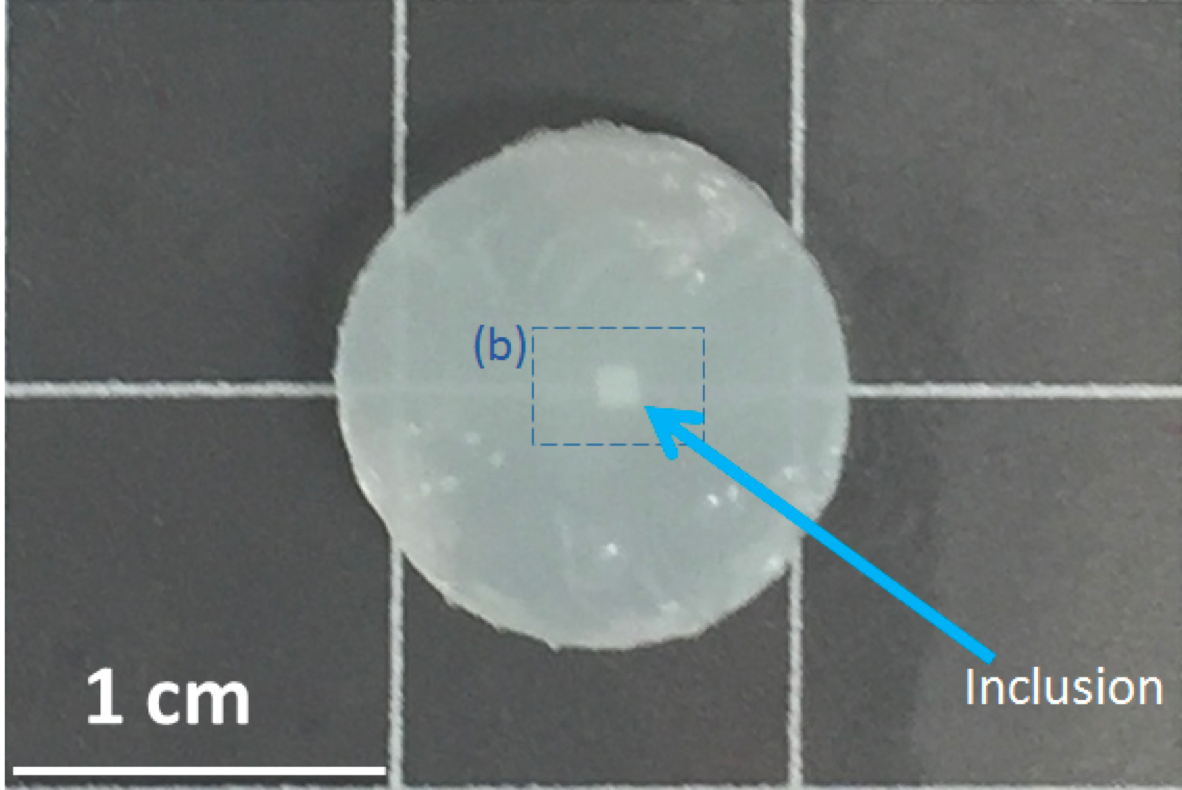
\includegraphics[width=\textwidth]{figures/phantom.png}
	\end{subfigure}
	\quad
	\begin{subfigure}{0.49\textwidth}
		\centering
		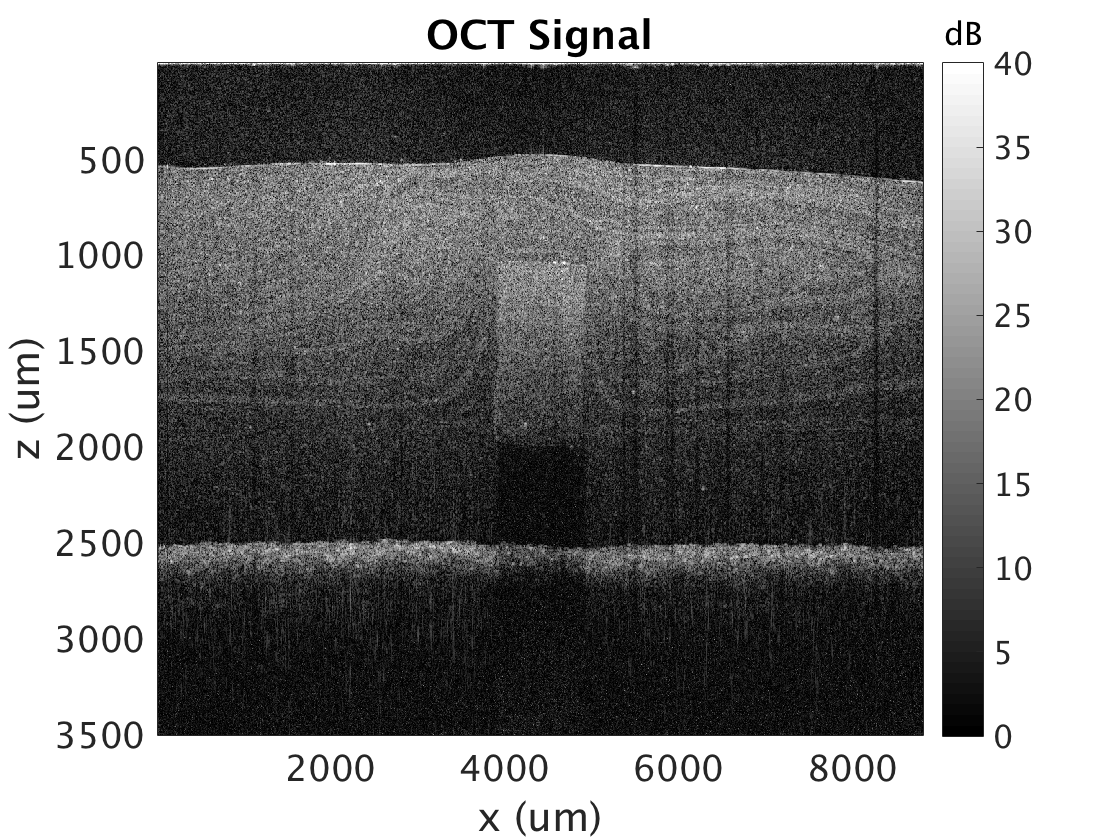
\includegraphics[width=\textwidth]{figures/oct.png}
	\end{subfigure}	
	\caption{The silicone phantom used to investigate strain estimation techniques a) photographed and b) imaged by the \ac{oct} system.}
	\label{oct_image}	
\end{figure}

To better quantify the image quality, an idealised silicone sample was imaged, to approximate breast tissue, and the strain estimated. This phantom consisted of a bulk, softer silicone material (with a Young's modulus of 6.4kPa) within which was a stiff, rectangular inclusion (Young's modulus of 100kPa) \cite{hepburn_improving_2017}, to which optical scatterers were added to enhance the \ac{oct} signal. The phantom was created by a previous Master's student, and was imaged using a desktop \ac{oce} system, with a system wavelength of $1300nm$. The imaged area, shown in \autoref{oct_image}, was divided into 2000 A-scans per each B-scan, over a length in x of $4.4\mu m$), and a total of 6817 B-scans were acquired, over the same length in y.

The complex \ac{oct} C-scan was initially processed from the raw spectral data produced by the Fourier-domain \ac{oct} system, to produce the complex \ac{oct} signal values, with associated optical amplitudes and random phase. From here, as described briefly in \autoref{compression_oce}, the difference in phase is calculated between loaded and unloaded B-scans, and averaged over 50 B-scan pairs. The strain estimation algorithms described following utilise this calculated averaged phase difference as the beginning step of the processing pipeline, and assume that the phase difference data is already loaded into memory.

\section{Strain Estimation Algorithms}\label{algorithms}

A total of six different strain estimation algorithms were implemented and tested, and can be differentiated based on how the phase unwrapping issue is addressed, and the digital differentiation filter used. \autoref{flowchart} demonstrates the decision processes in these strain estimation algorithms that separate the way they get from the complex phase difference delivered by the \ac{oct} system and pre-processing, to the final strain elastogram image.

The functions worked by using the complex phase difference C-scan as an input, as well as the specifications for the fit (axial) and lateral resolutions of the system. The fit resolution of the system determined the fit window for the \ac{wls} and \ac{sg} based strain estimation techniques, and the axial Gaussian $\sigma$ value for the \ac{fd} based techniques. The lateral resolution determined to what extent the strain images were laterally averaged by a Gaussian smoothing filter (for reasons discussed in the later section 4.3). If a lateral resolution of 0 was specified, no lateral smoothing was performed. 

\subsection{\ac{wls} with Unwrapped Phase}
The \ac{uwwls} algorithm unwraps the phase by reading in the entire volume and saves the unwrapped phase data to file. In a sequential loop over each B-scan the process reads in the complex phase and unwrapped phase for each B-scan. If lateral smoothing has been specified, it smooths the unwrapped phase using unweighted Gaussian smoothing by convoluting the unwrapped phase with the 1D lateral filter. A sequential looping is then performed over each A-scan and all fit segments within the given B-scan, which calculates the \ac{wls} estimate of strain using summations and the weights from the complex phase data.

\afterpage{

\begin{figure}[h!]
\begin{tikzpicture}[node distance=2cm, remember picture]
	\centering
	\node [anchor=north] at (0,0) (input) [io] {INPUT: $\Delta\phi_i$};
    
    \node (volume_unwrap) at (-4,-3) [basic] {Unwrapping Algorithm};
    \draw [wls] (input.225) edge[out=270,in=90] (volume_unwrap.100);
    \draw [uwsg] (input.240) edge[out=270,in=90] (volume_unwrap.80);
    
    \node (bscan_loop) at (0,-5.5) [main_long] {LOOP OVER B-SCANS};
    \draw [wls] (volume_unwrap.260) edge[out=270,in=90] (bscan_loop.135);
    \draw [uwsg] (volume_unwrap.280) edge[out=270,in=90] (bscan_loop.120);
    \draw [posg] (input.260)--(bscan_loop.100);
    \draw [wfd] (input.280)--(bscan_loop.80);
    \draw [uwfd] (input.300)--(bscan_loop.60);
    \draw [fdsm] (input.315)--(bscan_loop.45);
    
   	\node (variance) at (-4,-8) [basic] {Calculate variances};
    \draw [wls] (bscan_loop.225) edge[out=270,in=90] (variance.90);
    
    \node (unweighted) at (4,-8) [basic] {Remove phase weighting};
    \draw [uwfd] (bscan_loop.300) edge[out=270,in=90] (unweighted.90); 
    
    \node (lateral) at (0,-10.5) [temp] {LATERAL SMOOTHING};
    \draw [uwsg] (bscan_loop.240)--(lateral.120);
    \draw [posg] (bscan_loop.260)--(lateral.100);
    \draw [wfd] (bscan_loop.280)--(lateral.80);
    \draw [fdsm] (bscan_loop.315)--(lateral.45);

    \draw [wls] (variance.270) edge[out=270,in=90] (lateral.135);
    \draw [uwfd] (unweighted.270) edge[out=270,in=90] (lateral.60);
    
    \node (fit_loop) at (-4,-13.5) [main] {LOOP OVER FIT SEGMENTS};
    \draw [wls] (lateral.225) edge[out=270,in=90] (fit_loop.100);
    \draw [posg] (lateral.260) edge[out=270,in=90] (fit_loop.80);
    
    \node (ascan_loop) at (-6.5,-16) [main] {LOOP OVER A-SCANS};
    \draw [wls] (fit_loop.260) edge[out=270,in=90] (ascan_loop.90);
    
    \node (wls_strain) at (-4,-18) [basic] {WLS strain estimation};
    \draw [wls] (ascan_loop.270) edge[out=270,in=90] (wls_strain.90);
    
    \node (phase_offset) at (-2.5,-16) [basic] {Divide complex phase offset};
    \draw [posg] (fit_loop.280) edge[out=270,in=90] (phase_offset.90);
    
    \node (sg_filter) at (0,-18) [basic] {Convolve with SG Filter};
    \draw [posg] (phase_offset.270) edge[out=270,in=90] (sg_filter.100);
    \draw [uwsg] (lateral.240) edge[out=270,in=90] (sg_filter.120);
   
   \node (gauss_filter) at (2,-15.8) [basic] {Convolve with an axial 1D Gaussian filter};
   \draw [wfd] (lateral.280) edge[out=270,in=90] (gauss_filter.100);
   \draw [uwfd] (lateral.300) edge[out=270,in=90] (gauss_filter.80);
   
   \node (pre_filter) at (6,-15.5) [basic] {Convolve with a small 2D Gaussian 'pre-filter'};
   \draw [fdsm] (lateral.315) edge[out=270,in=90] (pre_filter.90);
   
   \node (fd) at (4,-18) [basic] {FD strain estimation};
   \draw [wfd] (gauss_filter.260) edge[out=270,in=90] (fd.80);
   \draw [uwfd] (gauss_filter.280) edge[out=270,in=90] (fd.60);
   \draw [fdsm] (pre_filter.270) edge[out=270,in=90] (fd.45);
   
   \node (output) at (0,-20.5) [io] {OUTPUT: $\epsilon$};
   \draw [wls] (wls_strain.270) edge[out=270,in=90] (output.135);
   \draw [uwsg] (sg_filter.240) edge[out=270,in=90] (output.120);
   \draw [posg] (sg_filter.260) edge[out=270,in=90] (output.100);
   \draw [wfd] (fd.280) edge[out=270,in=90] (output.80);
   \draw [uwfd] (fd.300) edge[out=270,in=90] (output.60);
   \draw [fdsm] (fd.315) edge[out=270,in=90] (output.45);

    % LEGEND:
   \matrix[draw=black,rounded corners] at (6,-1) {  
    \node (m1) at (0.5,0) [empty] {};
    \node (wls) at (3,0) [legendtext] {UW WLS};
    \draw [wls] (m1)--(wls.west);
    \node (m2) at (0.5,-0.5) [empty] {};
    \node (uwsg) at (3,-0.5) [legendtext] {UW SG};
    \draw [uwsg] (m2)--(uwsg.west);
    \node (m3) at (0.5,-1) [empty] {};
    \node (posg) at (3,-1) [legendtext] {PO SG};
    \draw [posg] (m3)--(posg.west);
    \node (m4) at (0.5,-1.5) [empty] {};
    \node (wfd) at (3,-1.5) [legendtext] {WFD};
    \draw [wfd] (m4)--(wfd.west);
    \node (m5) at (0.5,-2) [empty] {};
    \node (uwfd) at (3,-2) [legendtext] {UWFD};
    \draw [uwfd] (m5)--(uwfd.west);
    \node (m6) at (0.5,-2.5) [empty] {};
    \node (fdsm) at (3,-2.5) [legendtext] {PF FD};
    \draw [fdsm] (m6)--(fdsm.west);
    \\
    };

\end{tikzpicture}
\caption{Flowchart of pivotal processes for the six different strain estimation techniques investigated: unwrapping with \ac{wls} (blue), unwrapping with \ac{sg} filtering (orange), offset phase with \ac{sg} filtering (yellow), weighted smoothing with \ac{fd} (purple), unweighted smoothing with \ac{fd} (green), and pre-filtered \ac{fd} with weighted smoothing (light blue).}
\label{flowchart}
\end{figure}

\clearpage
}

\subsection{\ac{sg} Filtering on Unwrapped Phase}
The \ac{uwsg} unwraps the phase by the same process specified above, which requires a read from file of the unwrapped phase for each B-scan. If lateral smoothing required, the unwrapped phase is similarly smoothed via convolution with an unweighted Gaussian smoothing filter. To estimate the strain, this smoothed unwrapped phase data is convolved with the analytically derived \ac{sg} filter in a single action of the entire B-scan.
   
\subsection{\ac{sg} Filtering on Offset Phase}
In order to correct for phase unwrapping, the \ac{posg} function reads in the complex phase for each B-scan and loops over all fit segments within the B-scan, taking a matrix of values across all A-scans for the given depths. An averaged complex phase value for each fit segment is calculated and divided (corresponding to subtraction of the phase) to move the phase values into an unwrapped region. The \ac{sg} filter, which was pre-calculated using the analytical solution, is then convolved with the matrix in the axial direction to produce the strain estimation values at that given depth. 

\subsection{\ac{fd} on Weighted Smoothing of Phase Difference}
The \ac{wfd} smooths complex weighted phase difference that acts as the function's input using an axial Gaussian filter dependent on the fit resolution supplied (and a lateral filter if specified). For strain estimation, \ac{fd} is performed using bsxfun on the complex phase data (in order to prevent the introduction of  wrapping artefacts), by dividing one pixel by the conjugate of the previous pixel in order to subtract the phase values. This estimate of the spatial derivative of the phase difference is then converted into strain values.

\subsection{\ac{fd} on Unweighted Smoothing of Phase Difference}
This \ac{uwfd} algorithm works almost identically to the one described in the previous section, except that prior to using a Gaussian smoothing filter on the complex phase data, the amplitude is normalised to 1 for all phase difference values, effectively removing the optical weighting that comes from the OCT signal. From here the \ac{fd} is calculated, and from this the strain. 

\subsection{Pre-Filtered Phase Difference with Smoothed \ac{fd} Strain}

The \ac{pffd} algorithm was implemented as an effort to remove artefacts introduced by high intensity variable pixels in the \ac{wfd}. Using the weighted complex phase difference data, a small 2D Gaussian filter is applied to smooth out high intensity `speckle' pixels. This pre-filter is set at $20 \mu m$ resolution, approximately on the order of a few speckle. 
This action aims to counter the disproportionate influence of high intensity pixels over their neighbouring pixels, biasing the phase difference values towards them in the Kasai estimate. 
From here, the strain is estimated using \ac{fd}, and the resulting real strain is smoothed using a 2D Gaussian filter to match the required strain and lateral smoothing filter resolution values. 

The difference between this approach and the previous two \ac{fd} strain filter algorithms is the combination of a small, weighted smoothing filter to perform one operation (smooth out speckle) followed by the unweighted smoothing filter that compliments the derivative estimator.

Since the pre-filter contributes to the fit and lateral resolutions, for any given fit resolution $\text{FR}_{total}$ and lateral resolution $\text{LR}_{total}$ supplied to the function as input parameters, the resulting Gaussian smoothing resolutions must take into account the contribution from the pre-filter:

\begin{equation}
	\text{Res}_{Gauss} = \sqrt{\text{Res}_{total}^2 - \text{Res}_{pre}^2}
    \label{prefilter_res_FR}
\end{equation}

In order to maintain consistency between the strain estimation techniques, for the case in which no lateral smoothing is applied for any other algorithms, the pre-filter becomes 1D Gaussian smoothing filter only.

\autoref{strain_methods} summarises the six strain estimation techniques that have been developed, including the method with which they address the issue of phase unwrapping, and the strain filter they apply.

\begin{table}[h]
	\centering
	\begin{tabularx}{\textwidth}{YlYY}
		\toprule
		Name & Abbreviation & Phase Unwrapping & Strain Filter \\
		\midrule
		\ac{wls} with Unwrapped Phase & \ac{uwwls} & Volume unwrapping & \ac{wls} \\
		\ac{sg} Filtering on Unwrapped Phase & \ac{uwsg} & Volume unwrapping & \ac{sg} filter \\
		\ac{sg} Filtering on Offset Phase & \ac{posg} & Phase offset & \ac{sg} filter \\
		\ac{fd} on Weighted Smoothing of Phase & \ac{wfd} & None & \ac{fd} with (weighted) Gaussian smoothing \\
		\ac{fd} on Unweighted Smoothing of Phase & \ac{uwfd} & None & \ac{fd} with (unweighted) Gaussian smoothing \\
		Pre-Filtered Phase with Smoothed \ac{fd} & \ac{pffd} & None & Pre-filtering \& smoothing of \ac{fd} \\
		\bottomrule
	\end{tabularx}
	\caption{Description of the six strain estimation techniques investigated, including their abbreviation, and their method of tackling a) phase unwrapping and b) strain filtering.}
	\label{strain_methods}
\end{table}

\section{Phantom Strain Elastogram Results}\label{phantom_results}

\subsection{Qualitative Comparison}\label{qualitative1}

\begin{figure}[b!]
	\centering
    \begin{subfigure}{0.49\textwidth}
    	\centering
        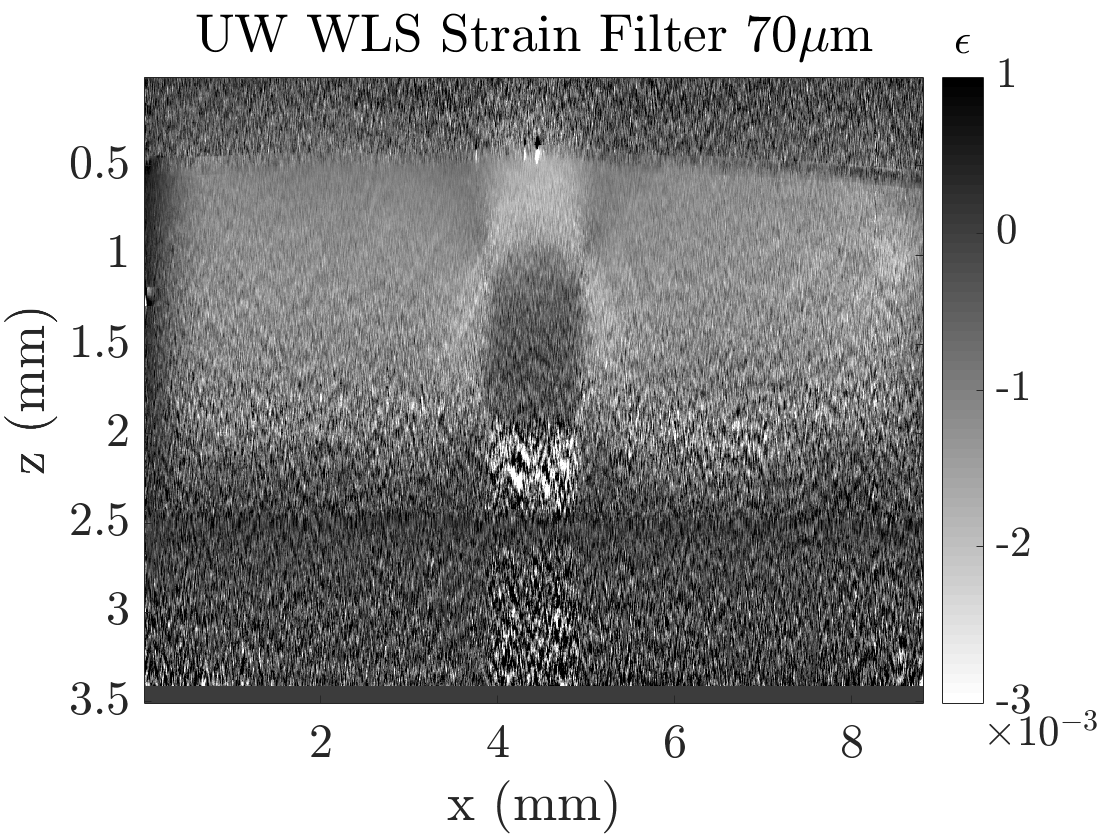
\includegraphics[width=\textwidth]{figures/wls_fr70_lr0.png}
	\end{subfigure}
    \begin{subfigure}{0.49\textwidth}
    	\centering
        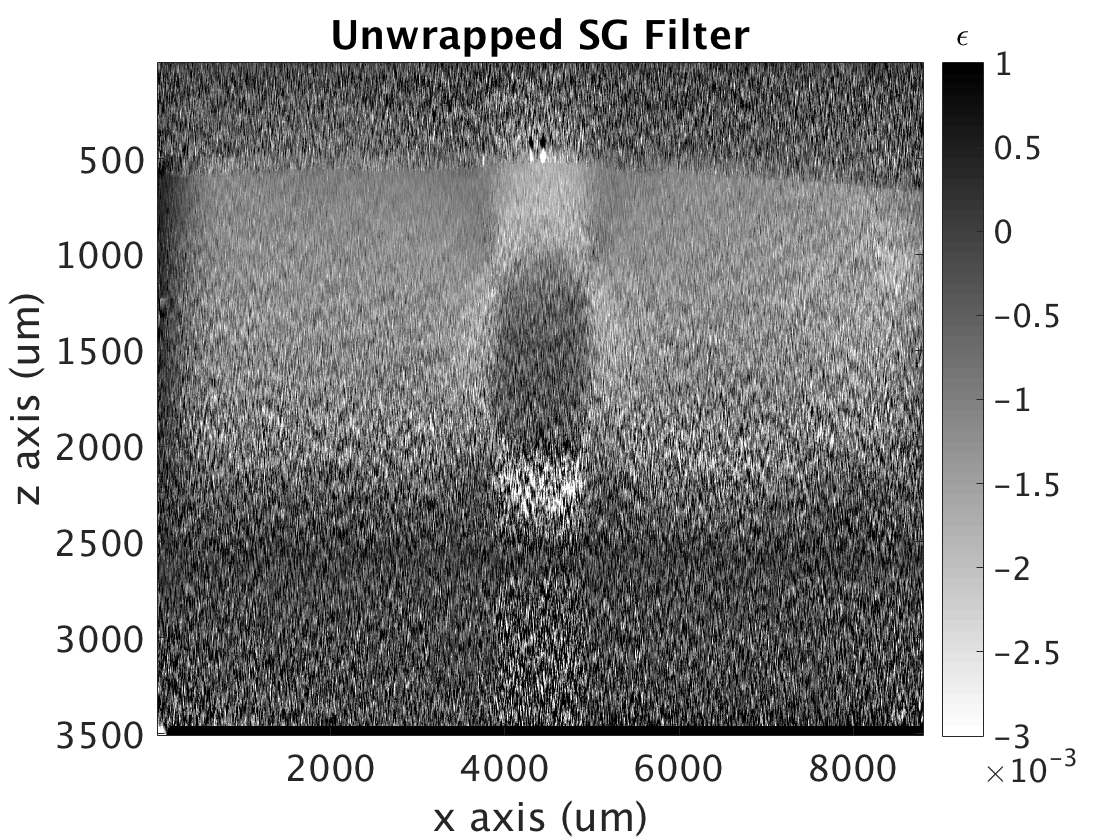
\includegraphics[width=\textwidth]{figures/uwsg_fr70_lr0.png}
	\end{subfigure}
    \\
    \begin{subfigure}{0.49\textwidth}
    	\centering
        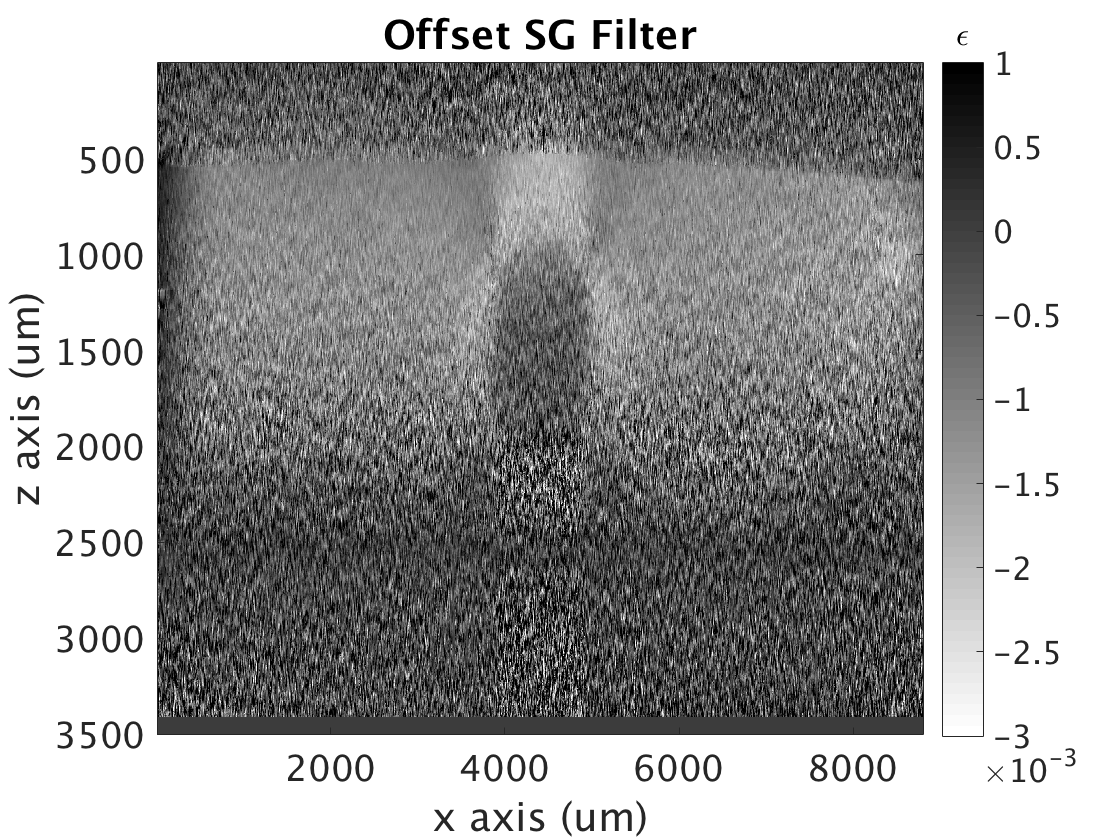
\includegraphics[width=\textwidth]{figures/posg_fr70_lr0.png}
	\end{subfigure}
    \begin{subfigure}{0.49\textwidth}
    	\centering
        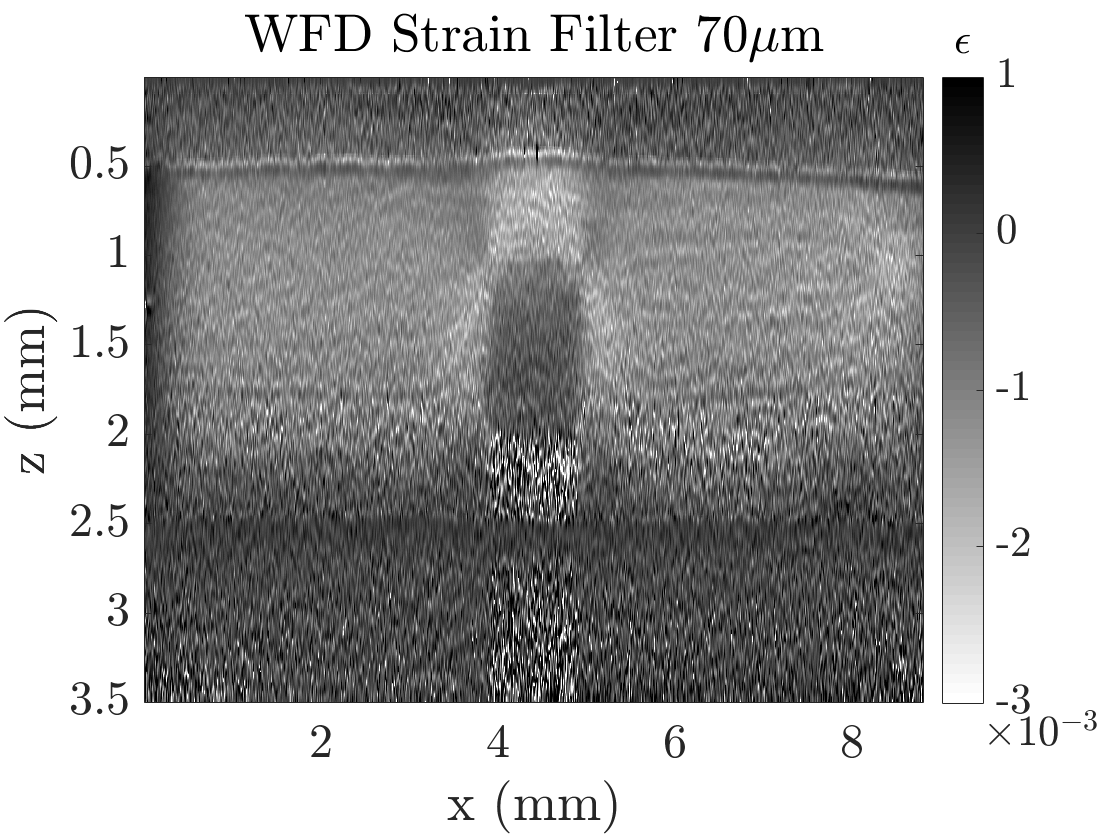
\includegraphics[width=\textwidth]{figures/wfd_fr70_lr0.png}
    \end{subfigure}
    \\
    \begin{subfigure}{0.49\textwidth}
    	\centering
        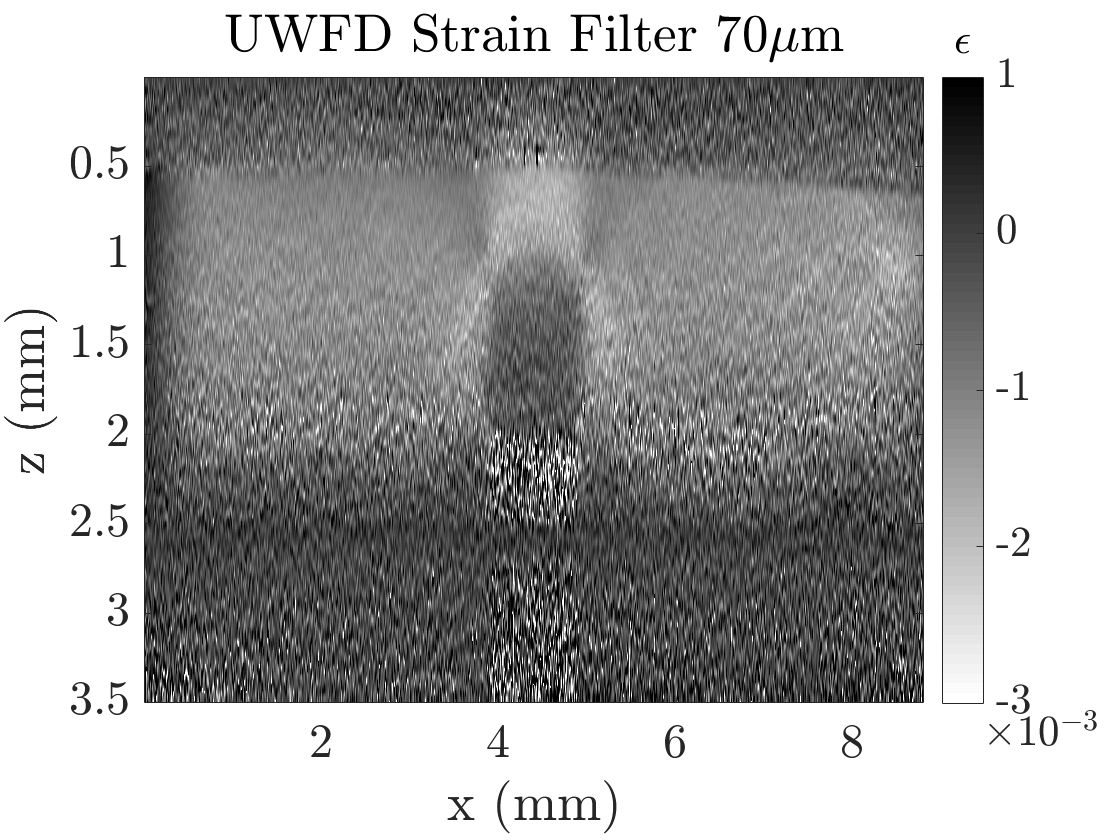
\includegraphics[width=\textwidth]{figures/uwfd_fr70_lr0.png}
	\end{subfigure}
    \begin{subfigure}{0.49\textwidth}
    	\centering
        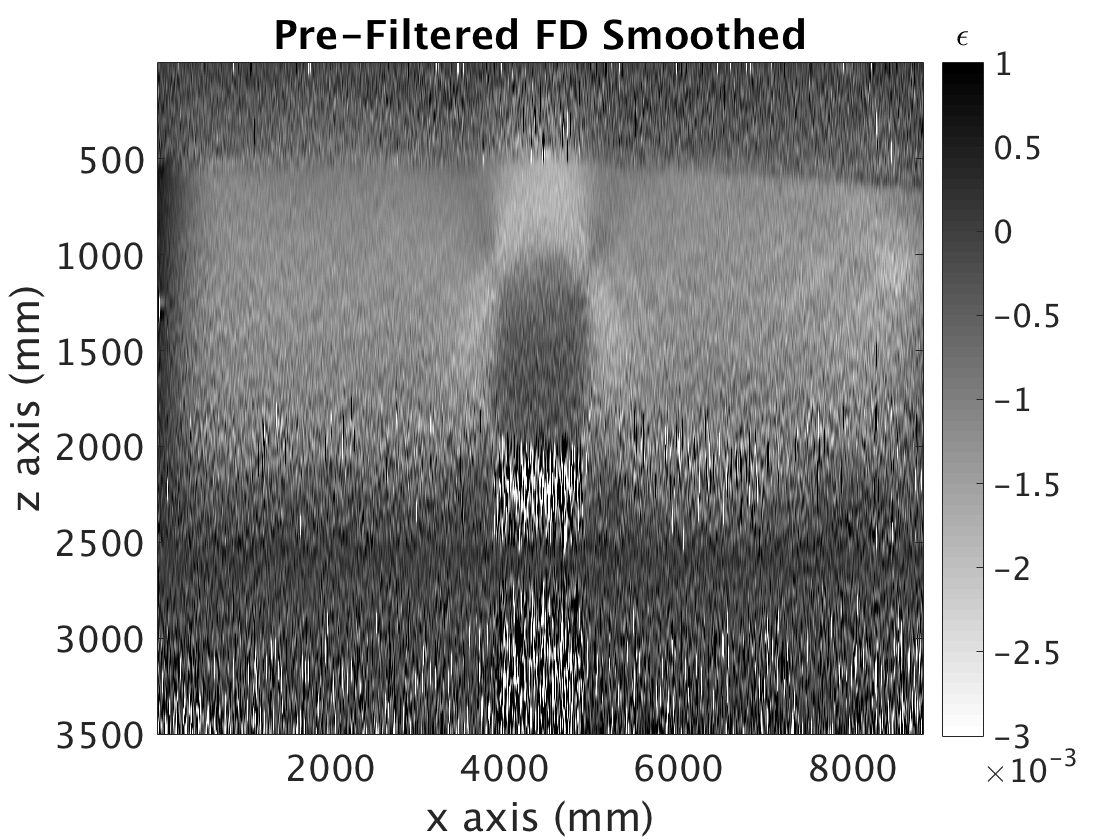
\includegraphics[width=\textwidth]{figures/fdsm_fr70_lr0.png}
    \end{subfigure}
	\caption{Strain B-scans taken from the centre of the phantom for the six strain estimation techniques discussed above, using a strain filter \ac{fwhm} of 70$\mu$m. The strain values shown are windowed between -3 and 1 milli-strain.}
    \label{bscan_images_1}	
\end{figure}

\autoref{bscan_images_1} shows the resulting B-scan strain images, taken from the centre of the phantom, for the six different strain estimation techniques described above. Note that negative strain corresponds to compressive force. The fact that there positive strain values exit suggests the assumption of uniaxial compression is invalid, as stiffer regions are pushing the softer bulk laterally and upwards. Alternatively, the $OCT_{SNR}<1$ in these regions.

In all images stiff inclusion shows less strain than the softer surrounding bulk, as expected. Around the inclusion in  all images, negative strain `haloes' are seen, caused by the stiff inclusion taking more of the compressive force than the soft bulk immediately next to it.
The area under the hard inclusion is characterised by low \ac{oct} signal, as can be seen in \autoref{oct_image}, and appears noisier in the techniques that utilise a phase unwrapping algorithm over the entire volume.
On a smaller scale, this pattern is seen in the same region in the weighted and unweighted smoothing of \ac{fd} strain, however it appears mostly removed in the \ac{posg} image.
The \ac{pffd} image has significant streak artefacts in this region. 

As mentioned before, the \ac{pffd} algorithm was introduced after noticing significant `ripple' effects in the \ac{wfd} algorithm. These can be seen prominently to the top right of the inclusion, and at a depth of approximately 1.8mm, and match with features in the \ac{oct} image in \autoref{oct_image}. In addition to this, the surface of the sample, which has a high reflectance and therefore strong optical weighting, becomes a prominent artefact in the \ac{wfd} image. The application of a small, weighted Gaussian pre-filter to this prior to unweighted Gaussian smoothing appears to have removed this issue, as well as slightly decreased the impact of the optical features at the top right, however at the expense of introducing a multitude of streak artefacts into the bottom half of the image in areas of low \ac{oct} signal.

\begin{figure}[t!]
	\centering
    \begin{subfigure}{0.49\textwidth}
    	\centering
        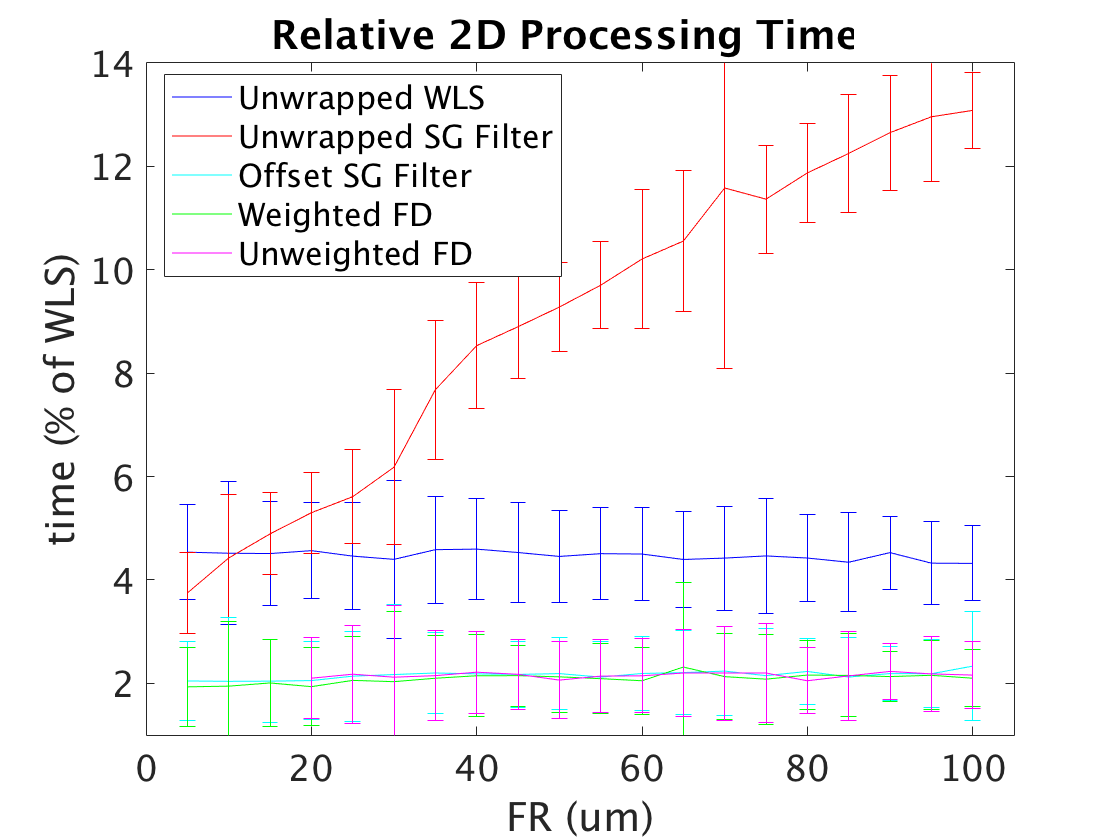
\includegraphics[width=\textwidth]{figures/2d_relative_fr.png}
    \end{subfigure}
    \begin{subfigure}{0.49\textwidth}
    	\centering
        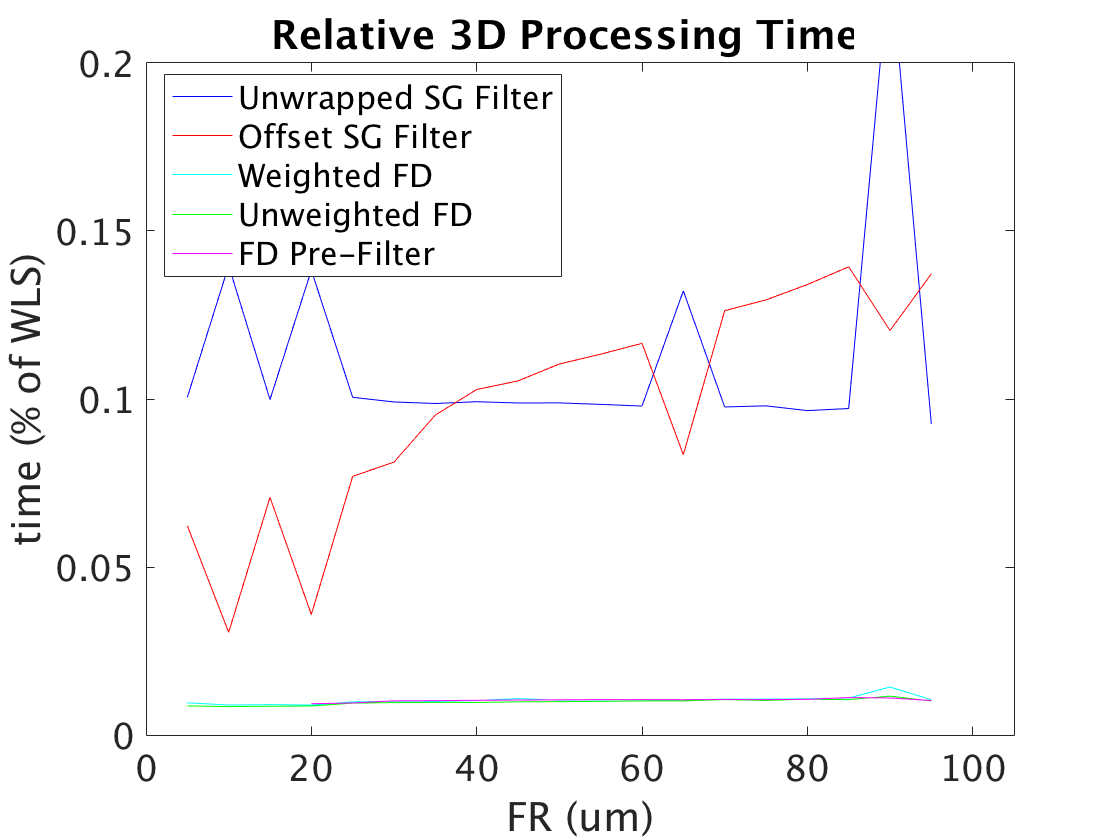
\includegraphics[width=\textwidth]{figures/3d_relative_fr.png}
    \end{subfigure}
    \caption{Relative processing time for different strain estimation techniques at different fit resolution values for a) a single B-scan and b) an entire C-scan. Error bars are the standard deviation of 50 repeated measurements.}
    \label{process_time_1}
\end{figure}

\subsection{Processing Time}

\autoref{process_time_1} shows the relative processing time for the different strain estimation techniques for both a single B-scan and an entire 3D C-scan, at different strain filter sizes. In order to compare accurately between the B-scan and C-scan, a 2D unwrapping algorithm was implemented instead of the usual 3D (which involves unwrapping across B-scans).
Each data point corresponds to an average of 20 processing time measurements. The error bars in the plot are the standard deviations of these 20 measurements. 
The relative processing time (with respect to \ac{uwwls}) is shown instead of the actual, to try provide an estimate that is comparable across different machines.
As a result of this, the standard deviation of the relative measurement is equal to the addition of the standard deviations of the absolute measurement and the baseline (\ac{uwwls}) measurement.
It can be seen that all new strain estimation techniques show a significant improvement in processing speed compared to the \ac{wls} estimate, and the \ac{fd} techniques in particular are much faster. 
The \ac{sg} filter on the unwrapped phase is faster than when applied to the phase offset, suggesting that the bottleneck caused by the non-linear subtraction operation contributes more to slowing the process down than needing to perform unwrapping on the entire volume. 

\subsection{Sensitivity}

\begin{figure}[b!]
	\centering
    \begin{subfigure}{0.49\textwidth}
    	\centering
        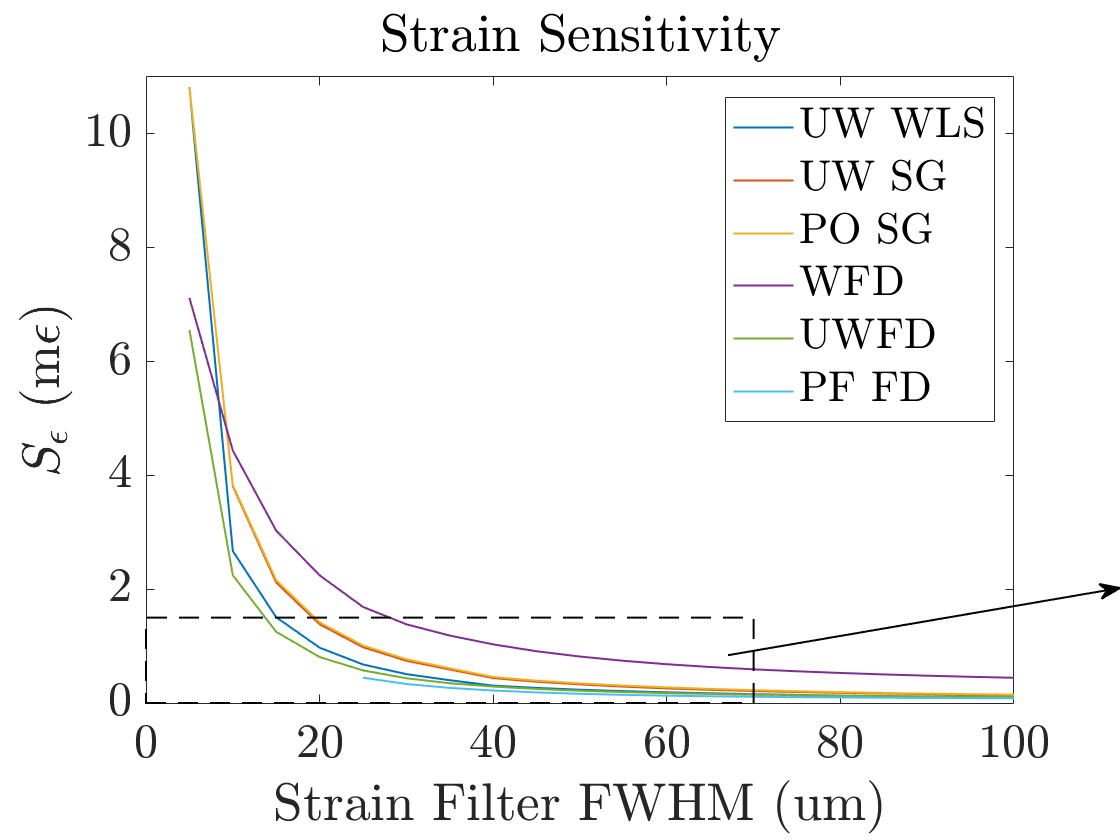
\includegraphics[width=\textwidth]{figures/sensitivity_lr0_arrow.png}
    \end{subfigure}
    \begin{subfigure}{0.49\textwidth}
    	\centering
        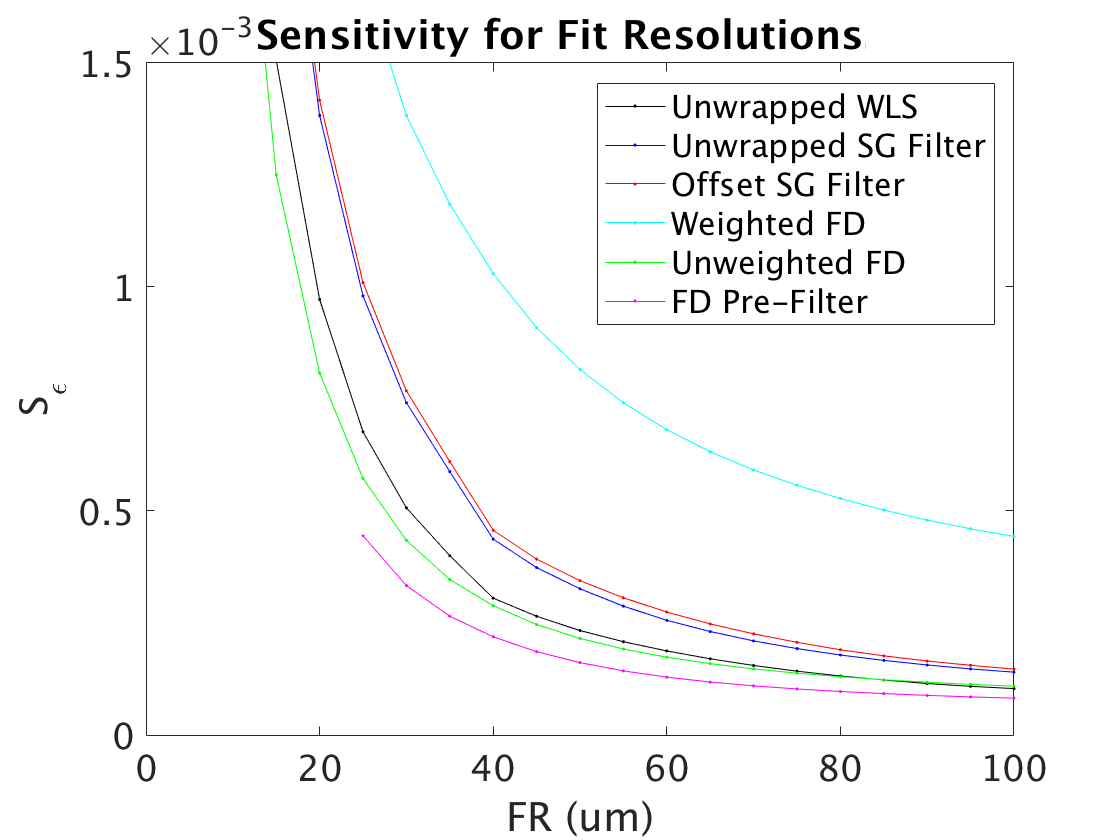
\includegraphics[width=\textwidth]{figures/sensitivity_lr0_zoom.png}
    \end{subfigure}
    \caption{Strain sensitivity values at different fit resolutions for all strain estimation techniques. The plot on the left is zoomed in to show the differences more clearly.}
	\label{sensitivity_1}
\end{figure}

The strain sensitivity for the six different estimation techniques across different strain filter \ac{fwhm} values is shown in \autoref{sensitivity_1}. There is a clear trend across all techniques, that for larger \ac{fwhm} values (corresponding to more smoothing) the sensitivity is better. 
The three techniques that offer the best sensitivity at lower fit resolutions are \ac{uwwls}, \ac{uwfd}, and \ac{pffd}. Of interest is the fact that the \ac{wfd} is significantly degraded compared to the other techniques, despite supposed to be weighting voxels with better quality information more highly.
The phase offset and unwrapping with \ac{sg} filtering are slightly worse than the \ac{wls} estimate, likely due to them being an \ac{ols} estimate, as opposed to a weighted one.
Although the pre-filtered \ac{fd} shows the best sensitivity as it has been defined in this work, it is important to note the artefacts present in the qualitative evaluation of the image. The sensitivity measurement is not indicative of the image quality as a whole, but only a segment of it.

On the basis of these results, it was decided to see if implementing lateral averaging over the separated B-scans could improve the sensitivity of the lower-order differentiation techniques (in particular the \ac{wfd} and those involving \ac{sg} filtering) towards that of the \ac{wls}. 

\section{Phantom Strain Elastogram Results with Lateral Averaging}\label{phantom_results_lateral}

\subsection{Qualitative Comparison}
It was found that very comparable image quality to higher strain filter \ac{fwhm} could be achieved using a smaller strain filter \ac{fwhm} of $40\mu m$ when lateral smoothing was also applied. \autoref{images} contains the B-scan  images for the different strain estimation techniques for selected strain and lateral smoothing filter \ac{fwhm} values. 

\subsection{Processing Time}

\begin{figure}[b!]
	\centering
    \begin{subfigure}{0.49\textwidth}
    	\centering
        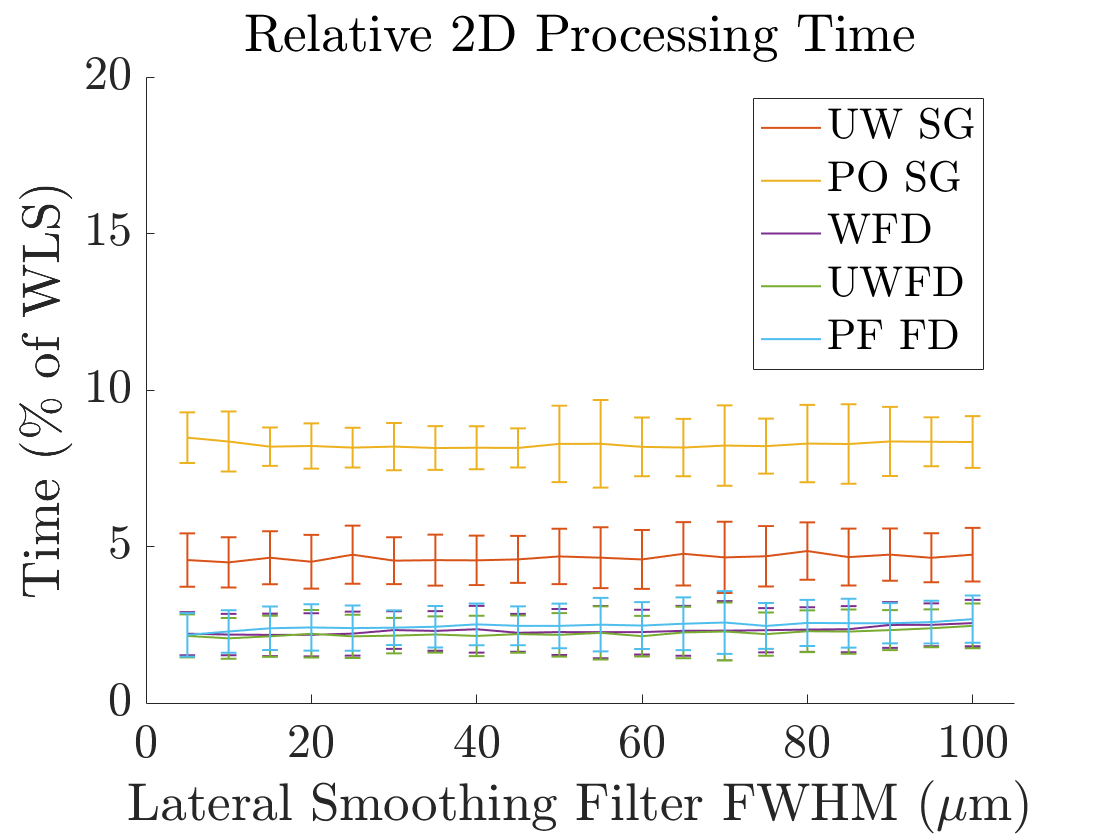
\includegraphics[width=\textwidth]{figures/2d_relative_lr.png}
    \end{subfigure}
    \begin{subfigure}{0.49\textwidth}
    	\centering
        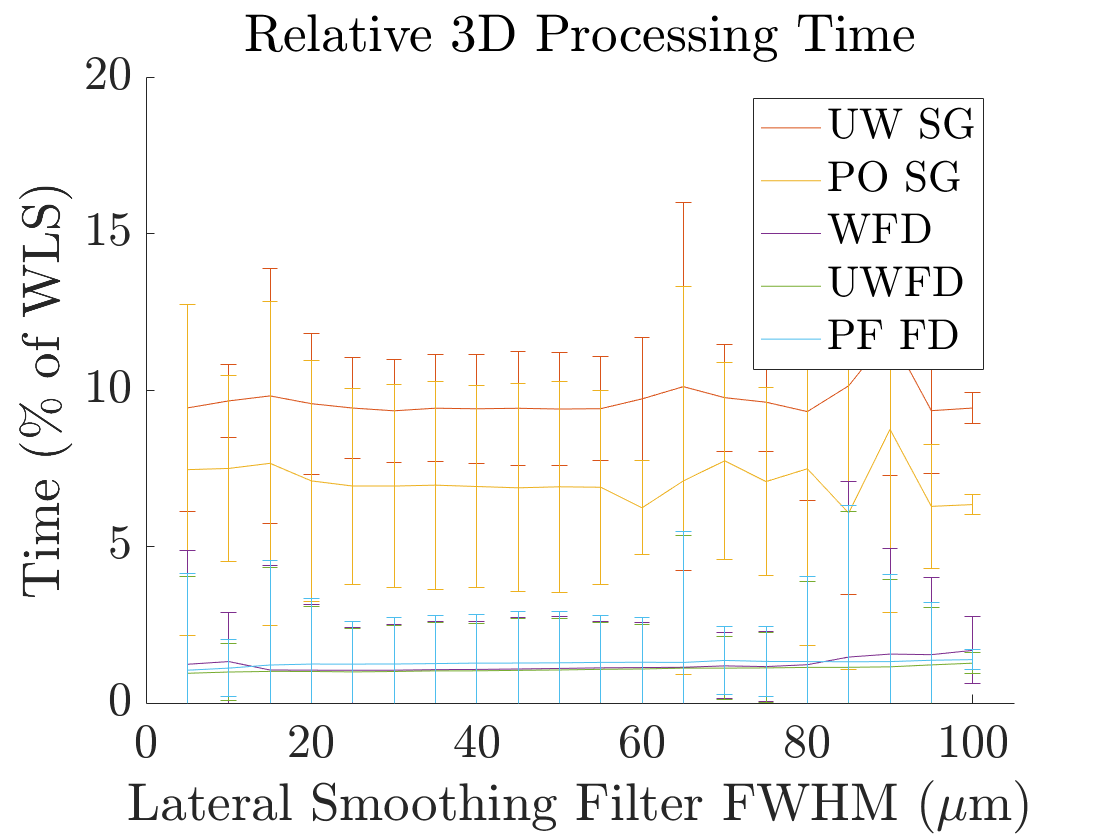
\includegraphics[width=\textwidth]{figures/3d_relative_lr.png}
    \end{subfigure}
	\caption{Relative processing time for different strain estimation techniques at a fit resolution of $40\mu m$ and with different lateral smoothing resolutions for a single B-scan and an entire C-scan.}
    \label{process_time_2}
\end{figure}

The benefit of adding lateral averaging is that it improves the sensitivity, and in most instances, without adding much time overhead, since it can be implemented as a 2D convolution on a given B-scan in the convolution algorithms (however not the \ac{uwwls}). Hence the focus of this section is largely on the image quality, rather than the processing time. However, \autoref{process_time_2} shows that adding lateral smoothing did not change the relative positions of the processing techniques in terms of processing time.

\subsection{Sensitivity}

The addition of lateral smoothing heightens the sensitivity of all imaging techniques. Using a base strain filter \ac{fwhm} of 40$\mu$m, \autoref{sensitivity_2} shows significant improvement in the sensitivity when lateral smoothing is applied, for all techniques.

\begin{figure}[t!]
	\centering
    \begin{subfigure}{0.49\textwidth}
    	\centering
        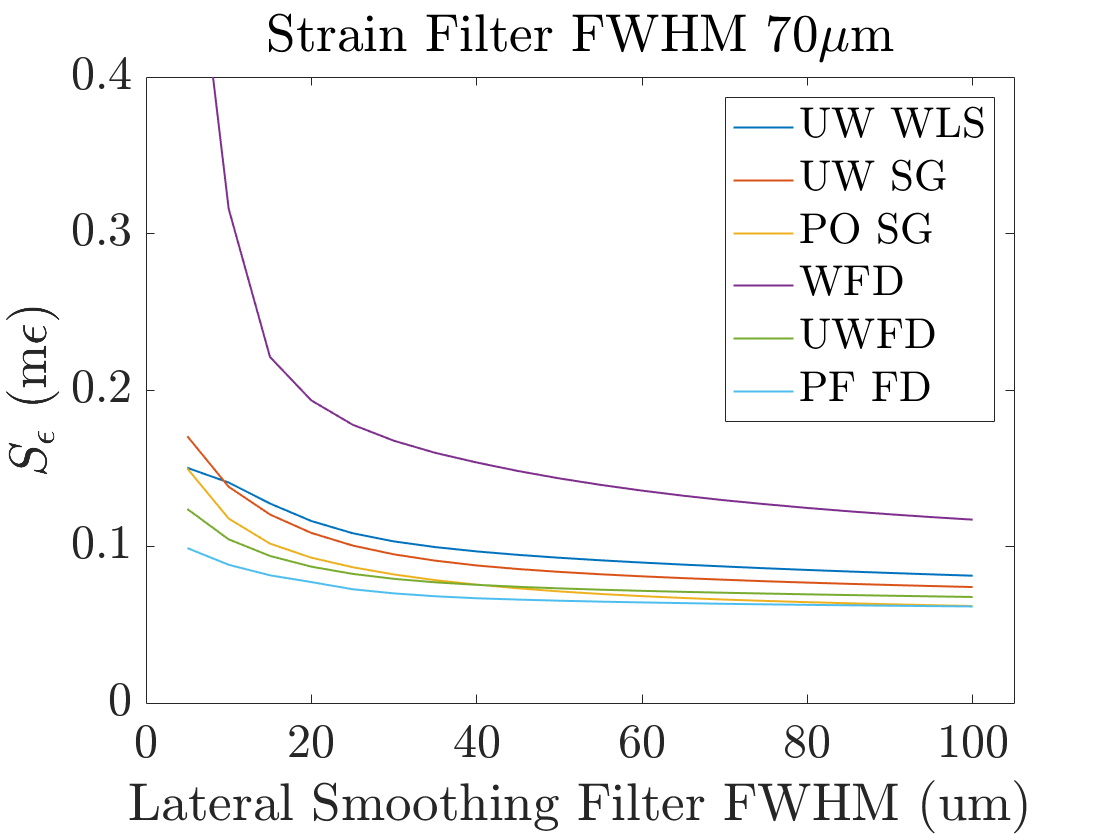
\includegraphics[width=\textwidth]{figures/sensitivity_fr70.png}
    \end{subfigure}
    \begin{subfigure}{0.49\textwidth}
    	\centering
        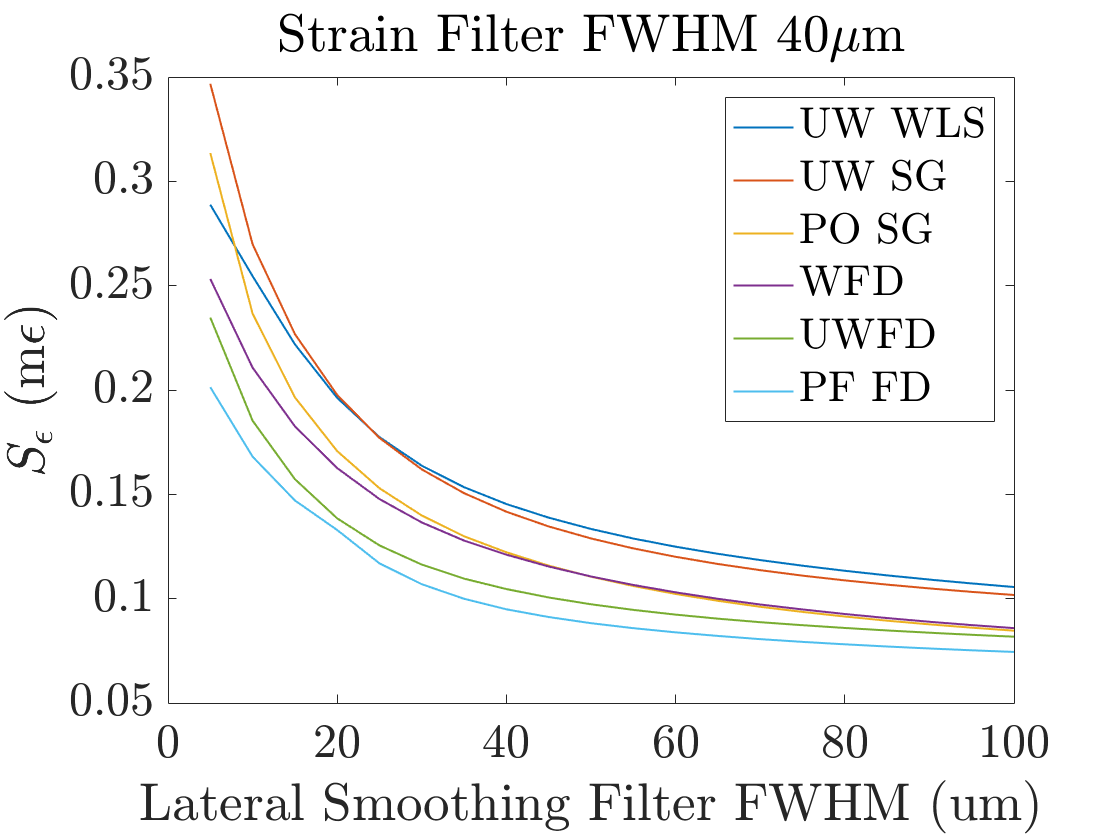
\includegraphics[width=\textwidth]{figures/sensitivity_fr40.png}
    \end{subfigure}
    \caption{Strain sensitivity for different lateral smoothing resolutions for a) Fit resolution of $70\mu m$, and b) $40\mu m$.}
    \label{sensitivity_2}	
\end{figure}

\begin{figure}[b!]
	\centering
	\begin{subfigure}{0.49\textwidth}
		\centering
		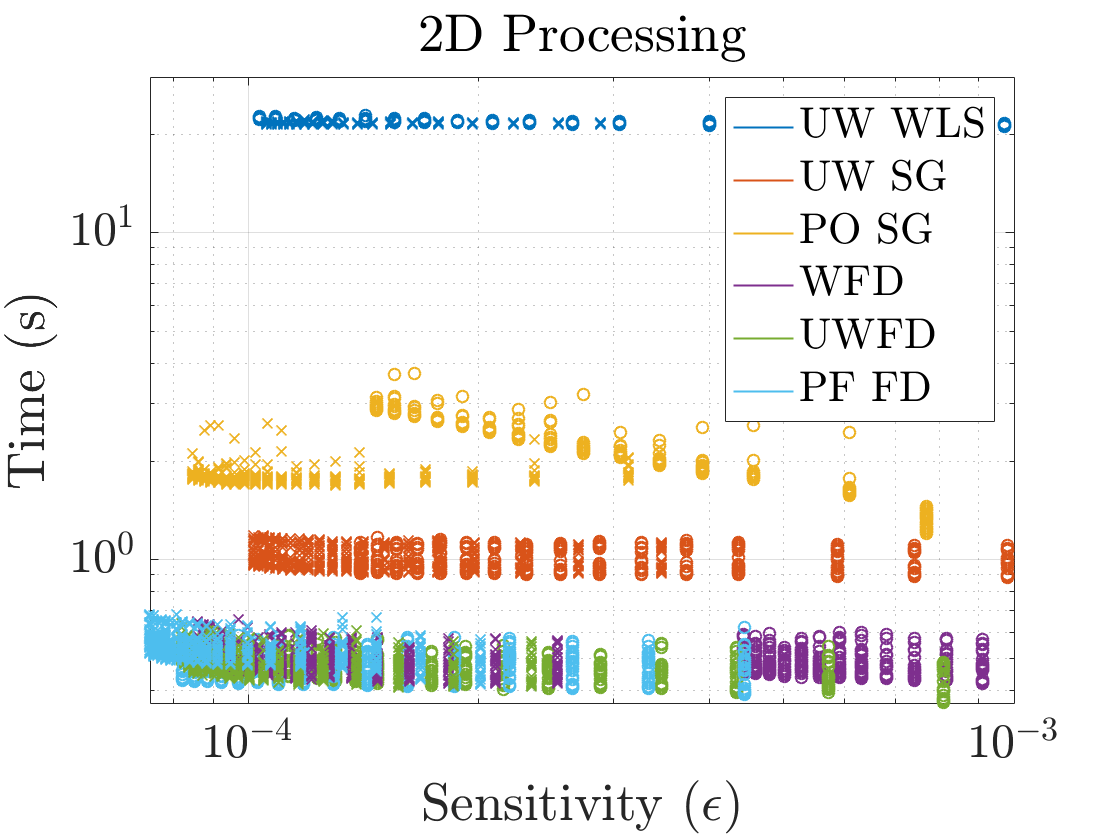
\includegraphics[width=\textwidth]{figures/sensitivity_2dtime.png}
	\end{subfigure}
	\begin{subfigure}{0.49\textwidth}
		\centering
		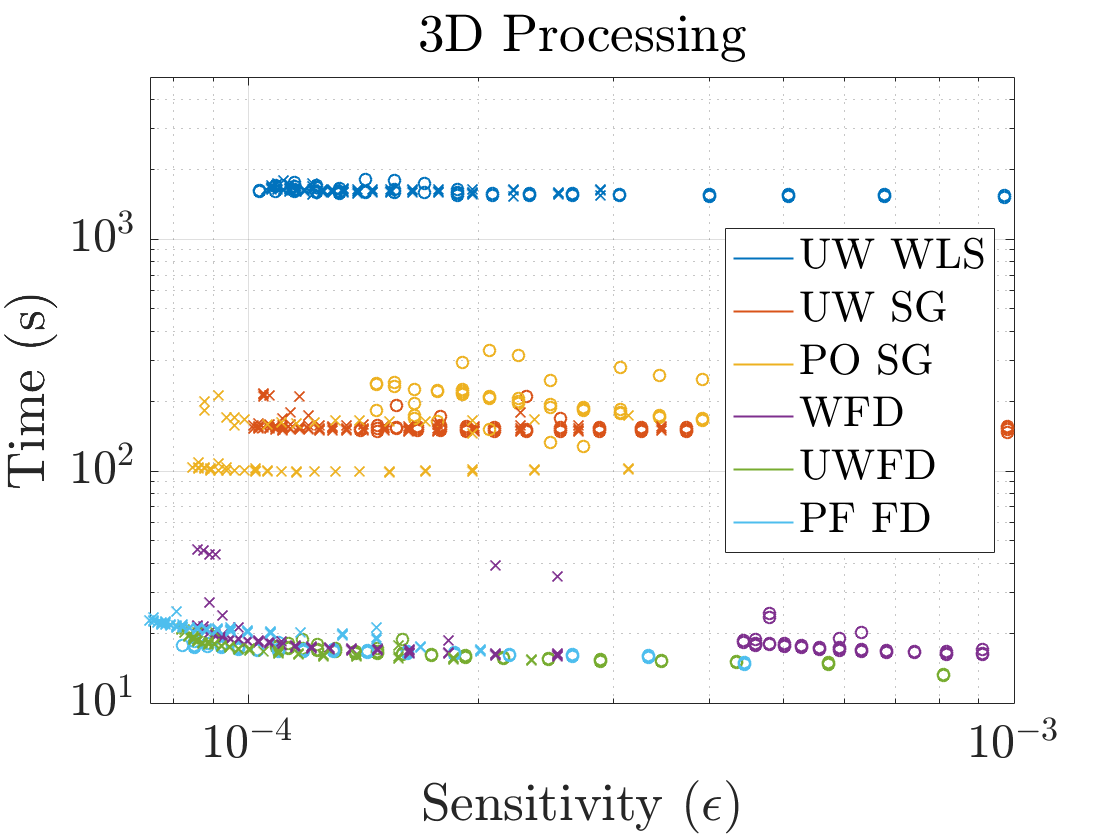
\includegraphics[width=\textwidth]{figures/sensitivity_3dtime.png}
	\end{subfigure}
	\caption{Absolute processing time in 2D and 3D for different sensitivity values based on differing strain filters (\textit{o})and lateral smoothing filters (\textit{x}) for the six strain estimation techniques, plotted on a log scale. The bottom left region of the plots corresponds to the optimum processing time and sensitivity values.}
	\label{sensitivity_time}
\end{figure}

\autoref{sensitivity_time} summarises the findings from the previous two sections. It has been shown that it is possible to greatly reduce the processing time by using \ac{fd} approaches, and that the sensitivity can be optimised by introducing lateral smoothing, which in most cases can be computed rapidly using a convolution operation. However, the overall image quality is not infinitely improved with more lateral smoothing and higher strain filter resolutions. The degradation of the resulting image resolution as a result of these processes, must also be examined.

\section{Analysis of Image Resolution} \label{image_res_results}

A goodness of fit limit was placed on the process of fitting an error function to the data set in order to calculate the image resolution, by requiring that the R-squared value of the fit must be over 0.5, which is quite low. This was justified by visually examining the fits, from which it was found that the high amounts of noise in the strain filter and lateral filters with low \ac{fwhm} degraded the R-squared value, while still producing a fit that maintained the trend in the data.
\autoref{imageres_figs} show density plots of the axial and lateral image resolution \ac{fwhm} for the different strain estimation techniques.

\begin{figure}[b!]
	\centering
	\begin{subfigure}{0.49\textwidth}
		\centering
		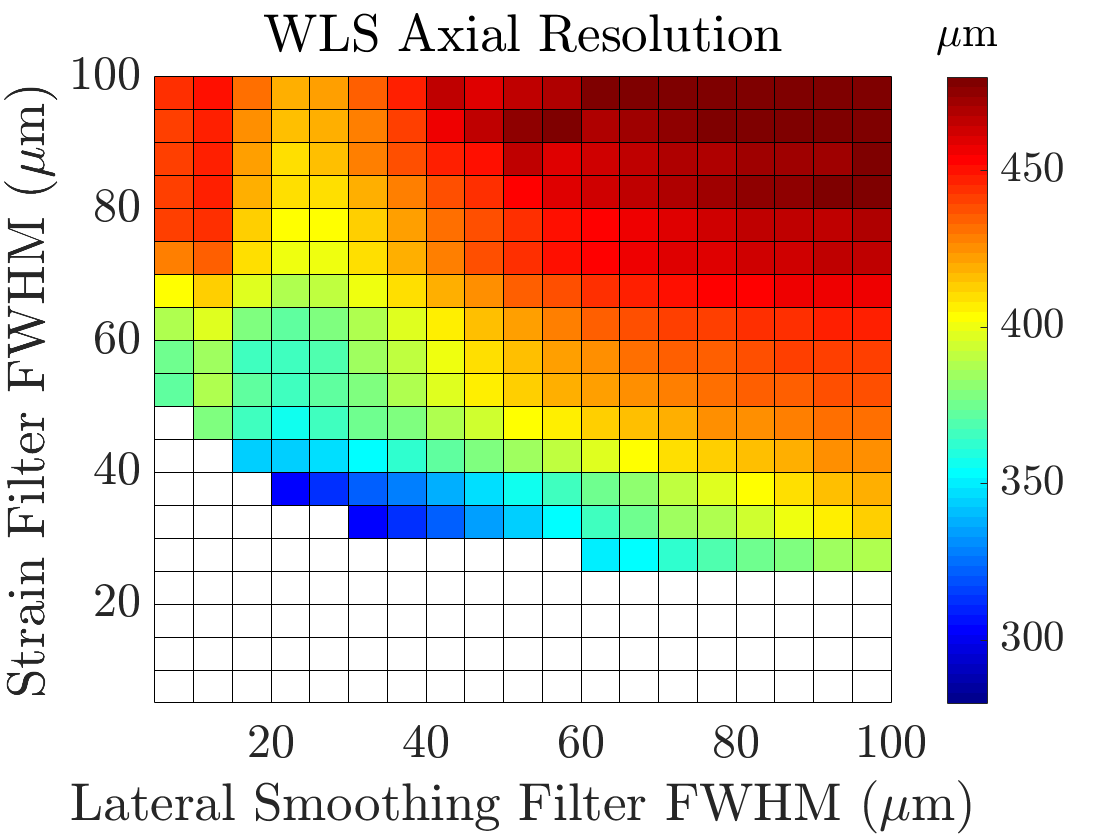
\includegraphics[width=\textwidth]{imageres_figs/wls_axial.png}
	\end{subfigure}
	\begin{subfigure}{0.49\textwidth}
		\centering
		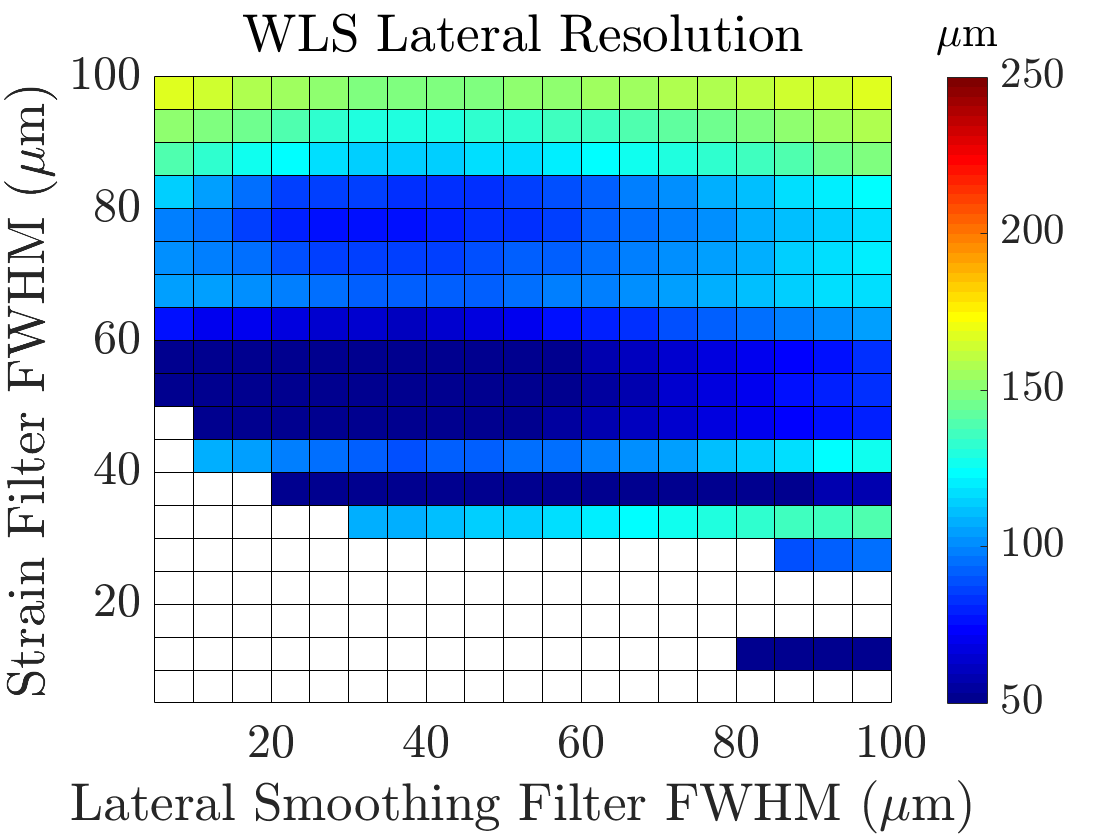
\includegraphics[width=\textwidth]{imageres_figs/wls_lateral.png}
	\end{subfigure}
	\\
	\begin{subfigure}{0.49\textwidth}
		\centering
		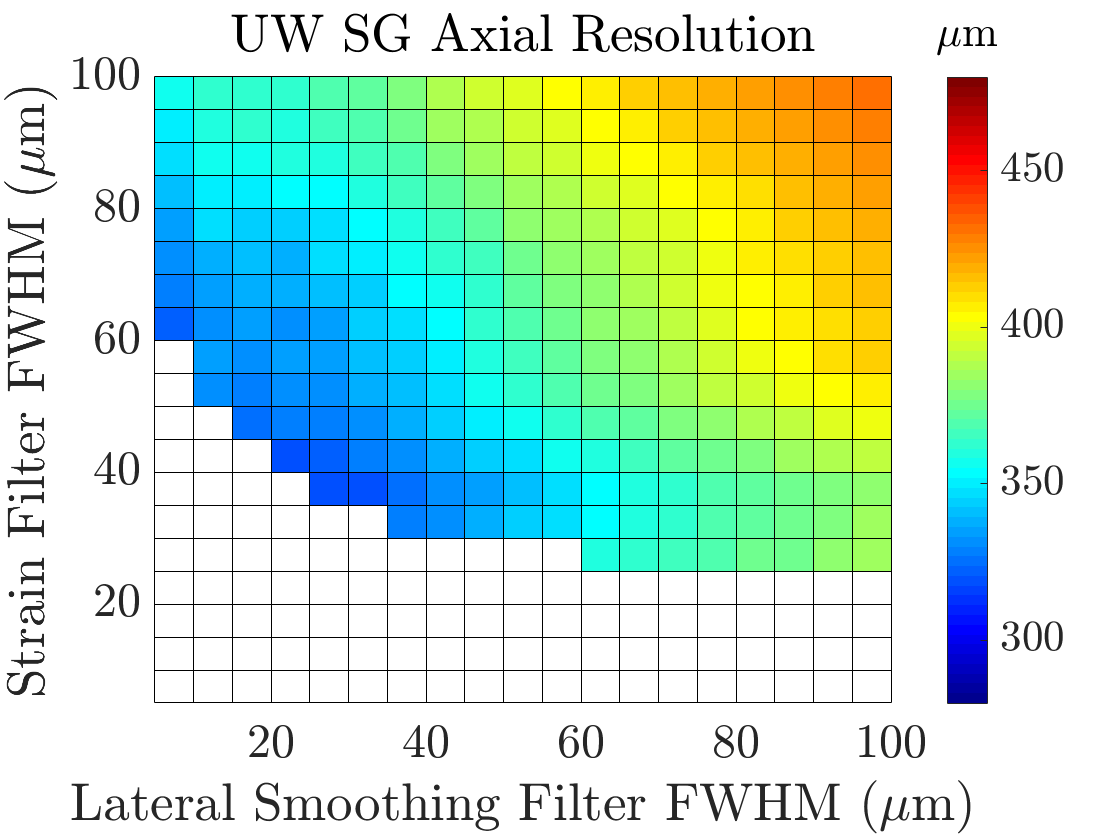
\includegraphics[width=\textwidth]{imageres_figs/uwsg_axial.png}
	\end{subfigure}
	\begin{subfigure}{0.49\textwidth}
		\centering
		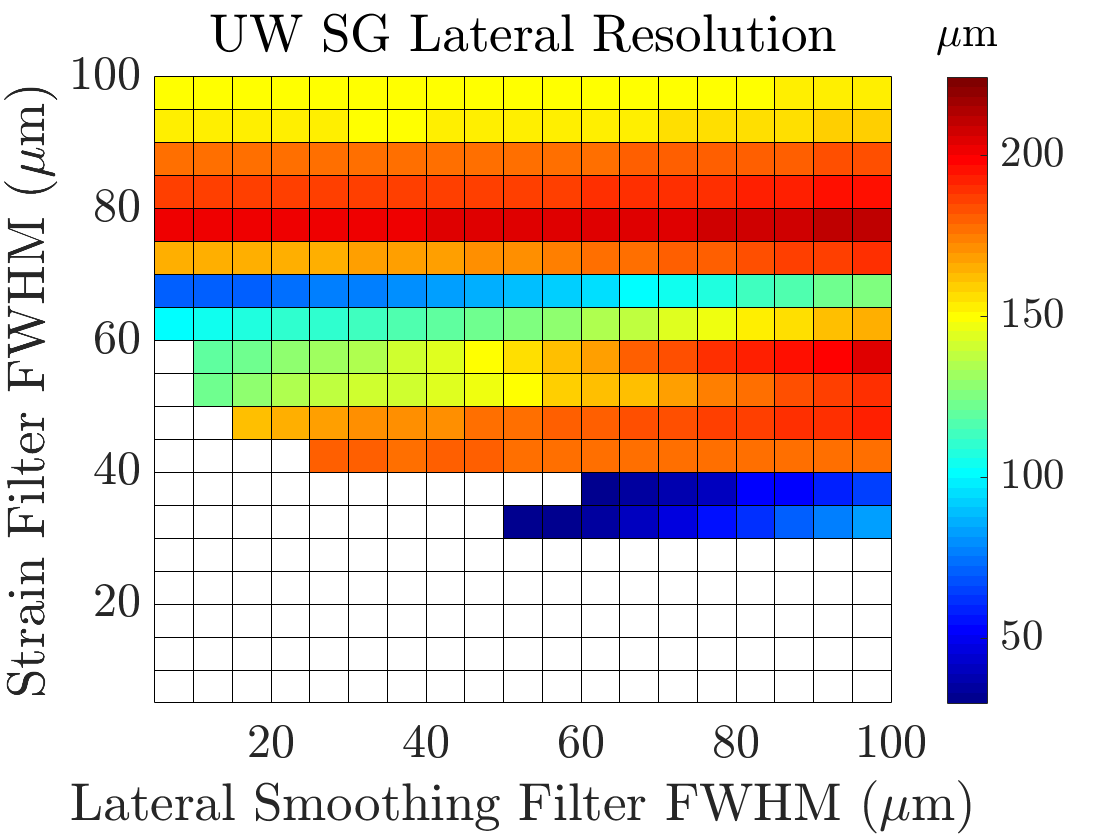
\includegraphics[width=\textwidth]{imageres_figs/uwsg_lateral.png}
	\end{subfigure}
	\\
\end{figure}

\afterpage{

\begin{figure}[h!]\ContinuedFloat	
	\begin{subfigure}{0.49\textwidth}
		\centering
		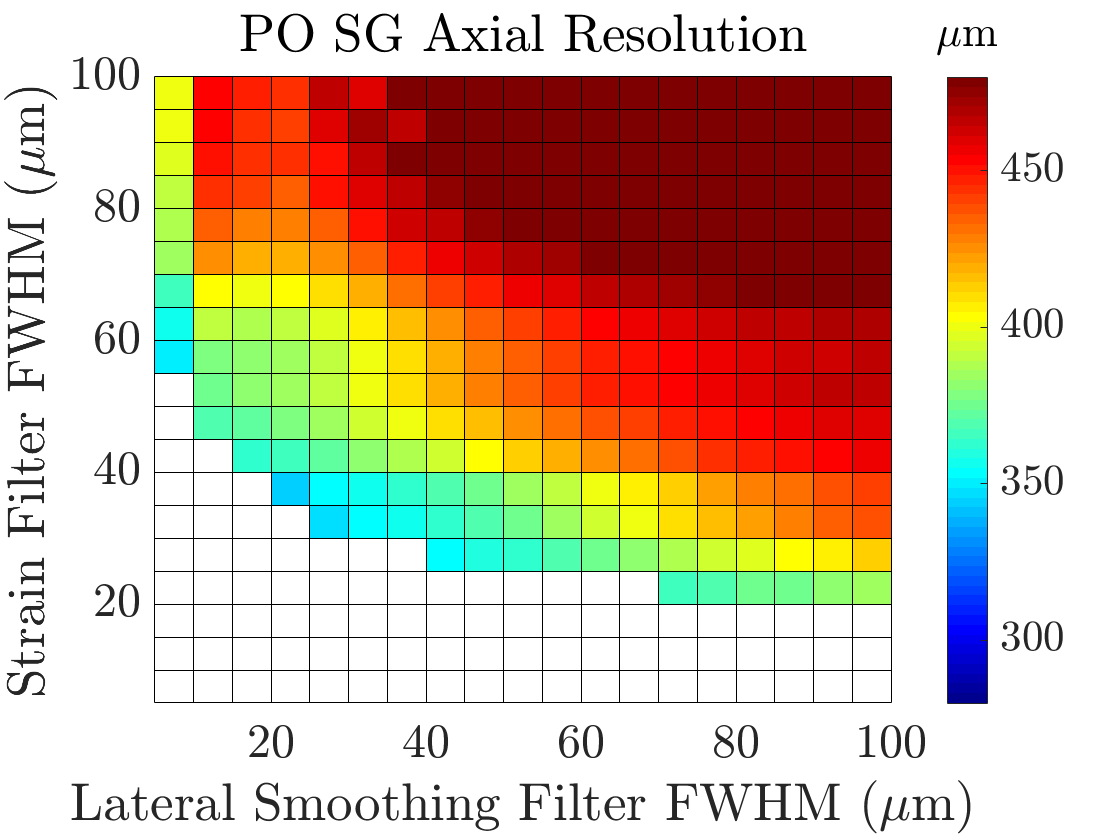
\includegraphics[width=\textwidth]{imageres_figs/posg_axial.png}
	\end{subfigure}
	\begin{subfigure}{0.49\textwidth}
		\centering
		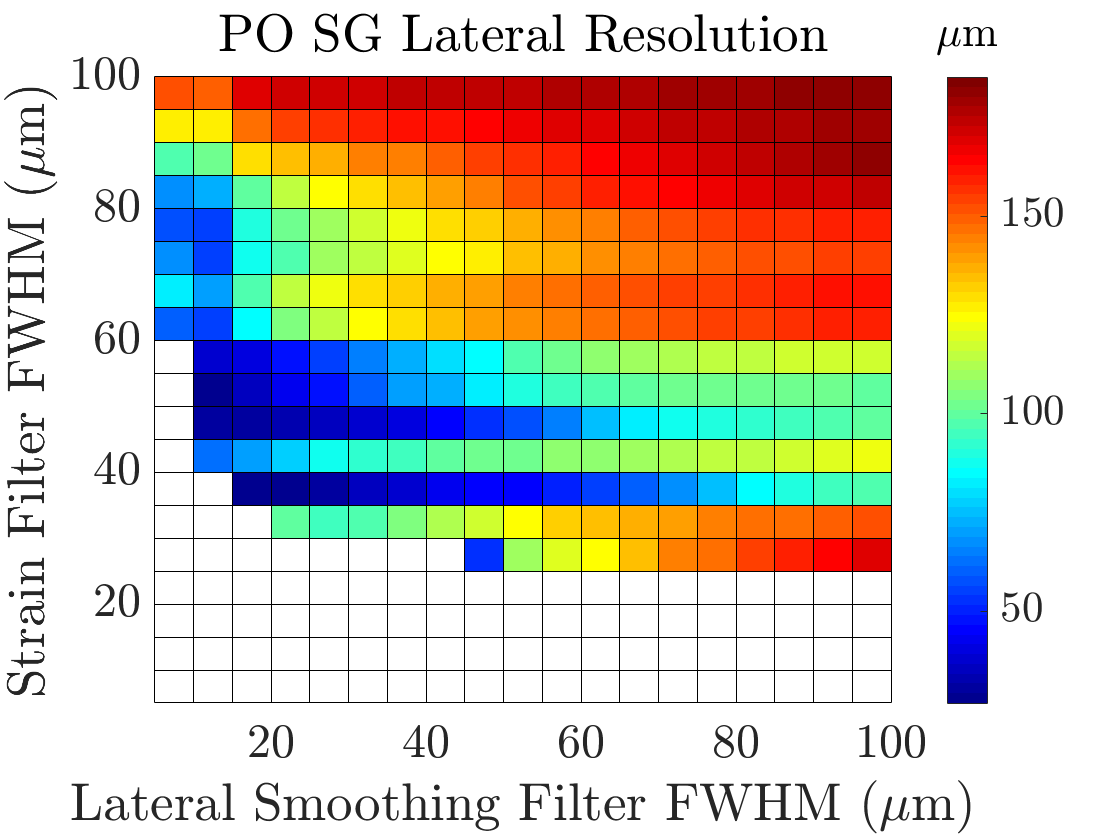
\includegraphics[width=\textwidth]{imageres_figs/posg_lateral.png}
	\end{subfigure}
	\\
	\begin{subfigure}{0.49\textwidth}
		\centering
		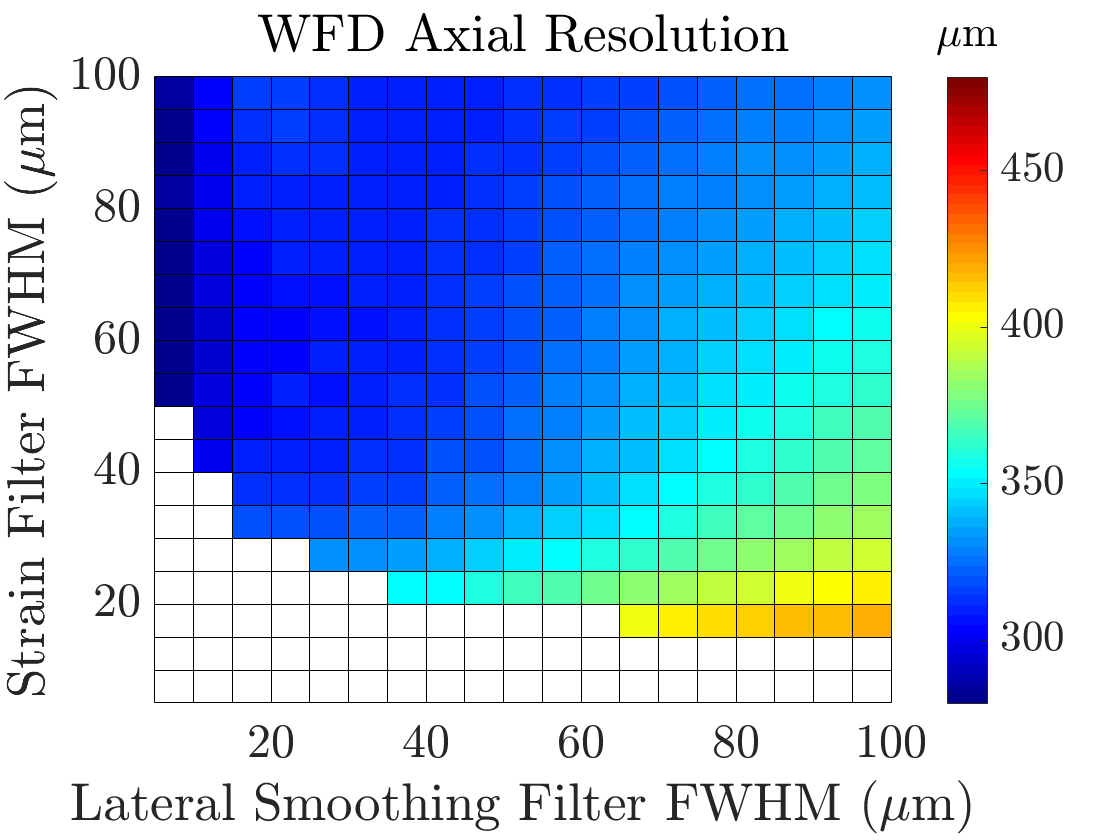
\includegraphics[width=\textwidth]{imageres_figs/wfd_axial.png}
	\end{subfigure}
	\begin{subfigure}{0.49\textwidth}
		\centering
		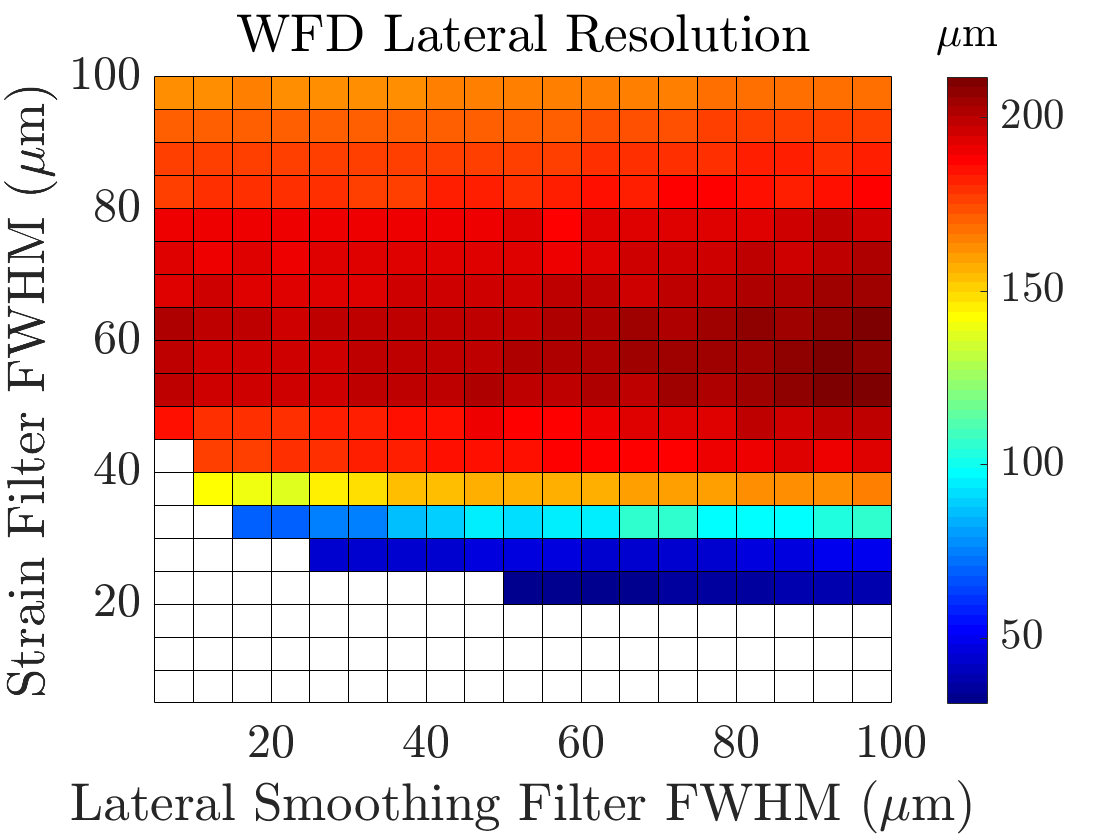
\includegraphics[width=\textwidth]{imageres_figs/wfd_lateral.png}
	\end{subfigure}
	\\
	\begin{subfigure}{0.49\textwidth}
		\centering
		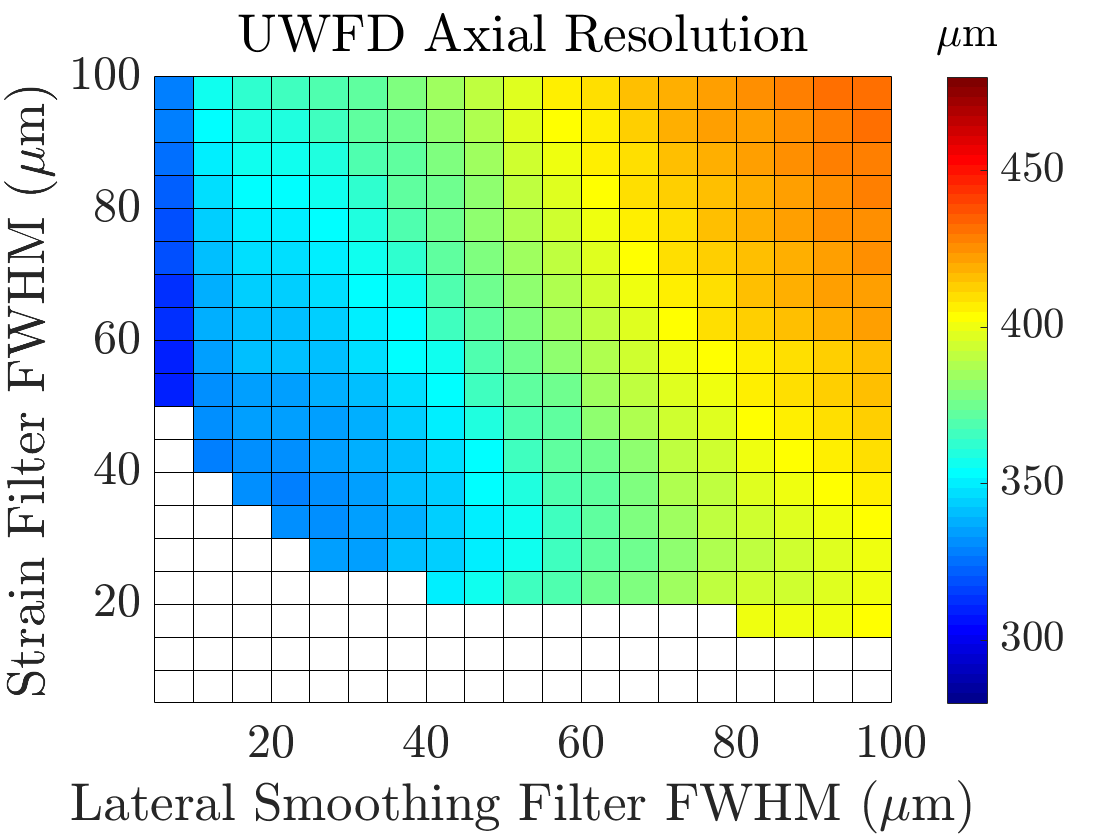
\includegraphics[width=\textwidth]{imageres_figs/uwfd_axial.png}
	\end{subfigure}
	\begin{subfigure}{0.49\textwidth}
		\centering
		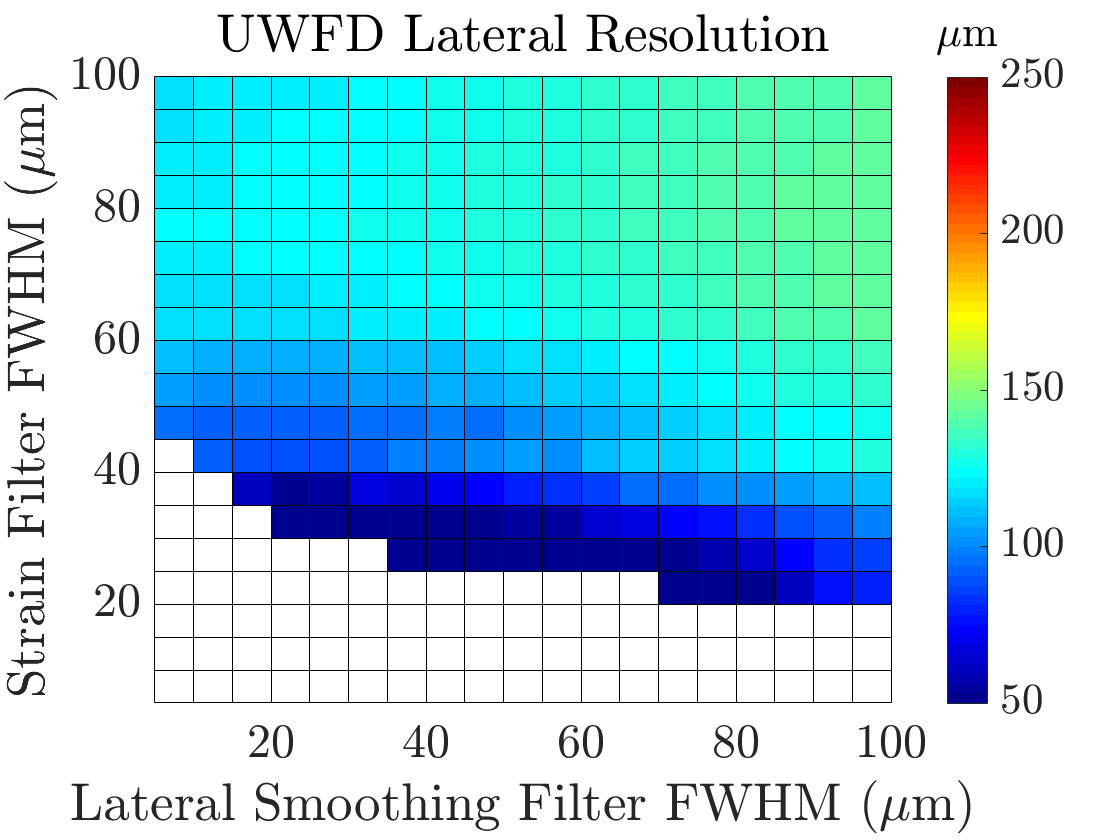
\includegraphics[width=\textwidth]{imageres_figs/uwfd_lateral.png}
	\end{subfigure}
	\\
	\begin{subfigure}{0.49\textwidth}
		\centering
		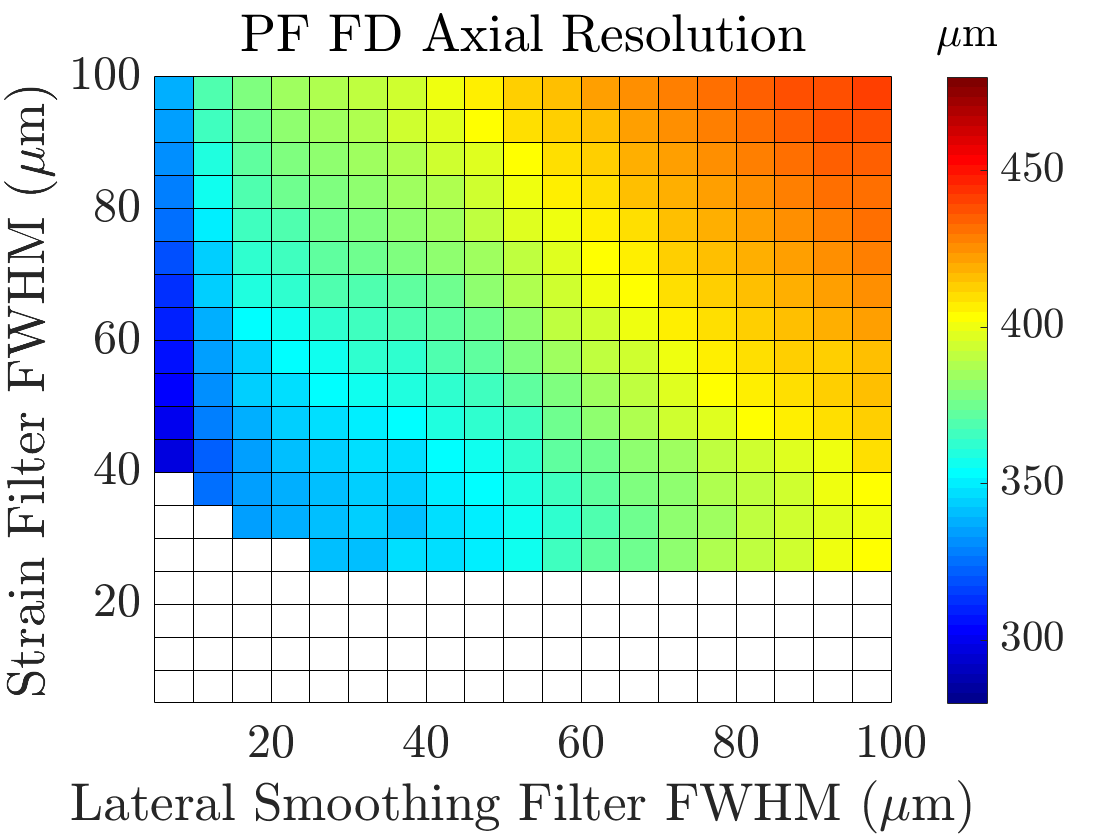
\includegraphics[width=\textwidth]{imageres_figs/pffd_axial.png}
	\end{subfigure}
	\begin{subfigure}{0.49\textwidth}
		\centering
		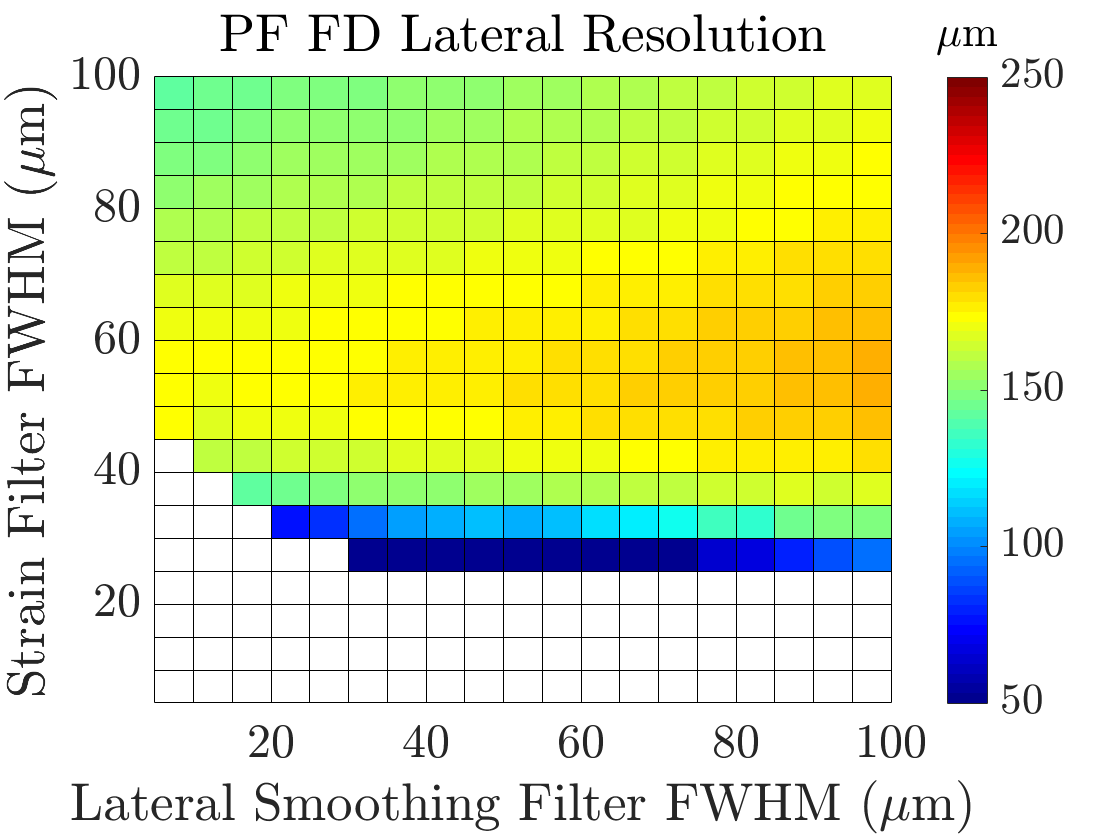
\includegraphics[width=\textwidth]{imageres_figs/pffd_lateral.png}
	\end{subfigure}
	\caption{The images on the left show the axial image resolution, and those on the right the lateral image resolution for the six different strain estimation techniques, at different strain and lateral smoothing filter \ac{fwhm} resolutions. Regions that are red correspond to worse image resolution.}
	\label{imageres_figs}
\end{figure}

\clearpage
}

\autoref{imageres_figs} show some interesting trends. The \ac{posg} algorithm performs the worst over both axial and lateral image resolution, with some reasonable lateral resolution for the mid-range strain filter \ac{fwhm}. The \ac{wfd} has a very poor lateral image resolution for any strain filter above approximately 40$\mu$m, however the axial resolution performs the best well in comparison to other techniques. The \ac{uwwls} strain filter is the opposite: it performs poorly for axial image resolution, however significantly better in the lateral resolution. 
This pattern contrasts to the other technique utilising phase unwrapping, \ac{uwsg}, suggesting the problem arises in the strain filtering process, and not the unwrapping algorithm. 
Both techniques that utilise \ac{sg} filtering have streak-like features in the lateral resolution at different strain filter \ac{fwhm} values, and are relatively poor. 
Both the \ac{uwfd} and \ac{pffd} show the best overall image resolution, with very similar axial resolution patterns, that are better at low strain and lateral smoothing filter \ac{fwhm} values (as would be expected). The \ac{pffd} however has slightly worse lateral resolution for higher strain and lateral smoothing filter \ac{fwhm}, in a pattern similar to that of the \ac{wfd} in these areas, but to a much lesser extent.

